% *****************************************************************************************************
% *******************      INTRO TO COMPETITIVE PROGRAMMING            ********************************
% *****************************************************************************************************

% =======================================================
% =======         HEADER FOR DOCUMENT        ============
% =======================================================
    
    % *********  SPECIFIC FOR THIS BOOK  ********
    \def\ProjectAuthorLink{https://github.com/CompilandoConocimiento}
    \def\ProjectNameLink{\ProjectAuthorLink/Reference}    
    

    % *********   DOCUMENT ITSELF   **************
    \documentclass[12pt, fleqn]{report}                             %Type of doc and size of font and left equations
    \usepackage[margin=1.2in]{geometry}                             %Margins and Geometry pacakge
    \usepackage{ifthen}                                             %Allow simple programming using if - then
    \usepackage[hidelinks]{hyperref}                                %Allow to create hiperlinks and Fuck Firefox
    \usepackage{pdfpages}                                           %Allow us 'import' PDF's
    \hypersetup{pageanchor=false}                                   %Solve 'double page 1' warnings in build :v
    \setlength{\parindent}{0pt}                                     %Eliminate ugly indentation
    \author{Oscar Andrés Rosas}                                     %Who I am

    % *********   LANGUAJE    *****************
    \usepackage[spanish]{babel}                                     %Please allow me to type in spanish
    \usepackage[utf8]{inputenc}                                     %Lets use UFT-8
    \usepackage[T1]{fontenc}                                        %Allow for better font support
    \usepackage{textcmds}                                           %Allow us to use quoutes
    \usepackage{changepage}                                         %Allow us to use identate paragraphs
    \usepackage{anyfontsize}                                        %All the sizes for fonts wiiiii!

    % *********   MATH AND HIS STYLE  *********
    \usepackage{ntheorem, amsmath, amssymb, amsfonts}               %All fucking math, I want all!
    \usepackage{mathrsfs, mathtools, empheq}                        %All fucking math, I want all!
    \usepackage{cancel}                                             %Negate symbol
    \usepackage{centernot}                                          %Allow me to negate a symbol
    \decimalpoint                                                   %Use decimal point

    % *********   GRAPHICS AND IMAGES *********
    \usepackage{graphicx}                                           %Allow to create graphics
    \usepackage{float}                                              %For images
    \usepackage{wrapfig}                                            %Allow to create images
    \graphicspath{ {Graphics/} }                                    %Where are the images :D

    % *********   LISTS AND TABLES ***********
    \usepackage{listings, listingsutf8}                             %We will be using code here
    \usepackage[inline]{enumitem}                                   %We will need to enumarate
    \usepackage{tasks}                                              %Horizontal lists
    \usepackage{longtable}                                          %Lets make tables awesome
    \usepackage{booktabs}                                           %Lets make tables awesome
    \usepackage{tabularx}                                           %Lets make tables awesome
    \usepackage{multirow}                                           %Lets make tables awesome
    \usepackage{multicol}                                           %Create multicolumns

    % *********   REMOVE SOME ERRORS **********
    \hbadness=10000                                                 %Ignore \vbox and \hbox warings
    \hfuzz=\maxdimen\newdimen\hfuzz                                 %Ignore \vbox and \hbox warings

    % *********   HEADERS AND FOOTERS ********
    \usepackage{fancyhdr}                                           %Lets make awesome headers/footers
    \pagestyle{fancy}                                               %Lets make awesome headers/footers
    \setlength{\headheight}{16pt}                                   %Top line
    \setlength{\parskip}{0.5em}                                     %Top line
    \renewcommand{\footrulewidth}{0.5pt}                            %Bottom line

    \lhead {                                                        %Left Header
        \hyperlink{chapter.\arabic{chapter}}                        %Make a link to the current chapter
        {\footnotesize{\textsc{\nouppercase{\leftmark}}}}           %And fot it put the name
    }

    \rhead {                                                        %Right Header
        \hyperlink{section.\arabic{chapter}.\arabic{section}}       %Make a link to the current chapter
            {\scriptsize{\textsc{\nouppercase{\rightmark}}}}        %And fot it put the name
    }

    \rfoot{\textsc{\small{\hyperref[sec:Index]{Ve al Índice}}}}     %This will always be a footer  

    \fancyfoot[L]{                                                  %Algoritm for a changing footer
        \ifthenelse{\isodd{\value{page}}}                           %IF ODD PAGE:
            {\href{https://SoyOscarRH.github.io/}                   %DO THIS:
                {\footnotesize                                      %Send the page
                    {\textsc{Oscar Andrés Rosas}}}}                 %Send the page
            {\href{https://compilandoconocimiento.com}              %ELSE DO THIS: 
                {\footnotesize                                      %Send the author
                    {\textsc{Compilando Conocimiento}}}}            %Send the author
    }
    
    
% =======================================================
% ===================   COMMANDS    =====================
% =======================================================

    % =========================================
    % =======   NEW ENVIRONMENTS   ============
    % =========================================
    \newenvironment{Indentation}[1][0.75em]                         %Use: \begin{Inde...}[Num]...\end{Inde...}
        {\begin{adjustwidth}{#1}{}}                                 %If you dont put nothing i will use 0.75 em
        {\end{adjustwidth}}                                         %This indentate a paragraph
    
    \newenvironment{SmallIndentation}[1][0.75em]                    %Use: The same that we upper one, just 
        {\begin{adjustwidth}{#1}{}\begin{footnotesize}}             %footnotesize size of letter by default
        {\end{footnotesize}\end{adjustwidth}}                       %that's it
    
    \def \Eq {equation}                                             %Stupid Visual studio error
    \newenvironment{MultiLineEquation}[1]                           %Use: To create MultiLine equations
        {\begin{\Eq}\begin{alignedat}{#1}}                          %Use: \begin{Multi..}{Num. de Columnas}
        {\end{alignedat}\end{\Eq}}                                  %And.. that's it!
    
    \newenvironment{MultiLineEquation*}[1]                          %Use: To create MultiLine equations
        {\begin{\Eq*}\begin{alignedat}{#1}}                         %Use: \begin{Multi..}{Num. de Columnas}
        {\end{alignedat}\end{\Eq*}}                                 %And.. that's it!

    \newenvironment{largeEq} {\begingroup \large}{\endgroup}        %Make eq bigger
    \newenvironment{LargeEq} {\begingroup \Large}{\endgroup}        %Make eq bigger
    \newenvironment{HugeEq} {\begingroup \Huge}{\endgroup}          %Make eq bigger!

    % =========================================
    % == GENERAL TEXT & SYMBOLS ENVIRONMENTS ==
    % =========================================
    
    % =====  TEXT  ======================
    \newcommand \Quote              {\qq}                           %Use: \Quote to use quotes
    \newcommand \Over               {\overline}                     %Use: \Bar to use just for short
    \newcommand \ForceNewLine       {$\Space$\\}                    %Use it in theorems for example
    \newcommand \ForceColumnBreak   {\vfill\null\columnbreak}       %Use only in multicols
    \newcommand \Link[2] {\underline{\textCode{\href{#1}{#2}}}}       %Use a link

    % =====  SPACES  ====================
    \DeclareMathOperator \Space     {\quad}                         %Use: \Space for a cool mega space
    \DeclareMathOperator \MegaSpace {\quad \quad}                   %Use: \MegaSpace for a cool mega mega space
    \DeclareMathOperator \MiniSpace {\;}                            %Use: \Space for a cool mini space
    
    % =====  MATH TEXT  =================
    \newcommand \Such           {\MiniSpace | \MiniSpace}           %Use: \Such like in sets
    \newcommand \Also           {\MiniSpace \text{y} \MiniSpace}    %Use: \Also so it's look cool
    \newcommand \Remember[1]    {\Space\text{\scriptsize{#1}}}      %Use: \Remember so it's look cool
    
    % =====  THEOREMS: IN SPANISH :0  ===
    \newtheorem{Theorem}        {Teorema}[section]                  %Use: \begin{Theorem}[Name]\label{Nombre}...
    \newtheorem{Corollary}      {Colorario}[Theorem]                %Use: \begin{Corollary}[Name]\label{Nombre}...
    \newtheorem{Lemma}[Theorem] {Lemma}                             %Use: \begin{Lemma}[Name]\label{Nombre}...
    \newtheorem{Definition}     {Definición}[section]               %Use: \begin{Definition}[Name]\label{Nombre}...
    \theoremstyle{break}                                            %THEOREMS START 1 SPACE AFTER Fuck!

    % =====  LOGIC  =====================
    \newcommand \lIff    {\leftrightarrow}                          %Use: \lIff for logic iff
    \newcommand \lEqual  {\MiniSpace \Leftrightarrow \MiniSpace}    %Use: \lEqual for a logic double arrow
    \newcommand \lInfire {\MiniSpace \Rightarrow \MiniSpace}        %Use: \lInfire for a logic infire
    \newcommand \lLongTo {\longrightarrow}                          %Use: \lLongTo for a long arrow
    \newcommand \lAnd    {\land}                                    %Use: \lAnd ^
    \newcommand \lOr     {\lor}                                     %Use: \lOr or symbol
    \newcommand \lNot    {\neg}                                     %Use: \lNot for negation

    % =====  FAMOUS SETS  ===============
    \DeclareMathOperator \Naturals     {\mathbb{N}}                 %Use: \Naturals por Notation
    \DeclareMathOperator \Primes       {\mathbb{P}}                 %Use: \Primes por Notation
    \DeclareMathOperator \Integers     {\mathbb{Z}}                 %Use: \Integers por Notation
    \DeclareMathOperator \Racionals    {\mathbb{Q}}                 %Use: \Racionals por Notation
    \DeclareMathOperator \Reals        {\mathbb{R}}                 %Use: \Reals por Notation
    \DeclareMathOperator \Complexs     {\mathbb{C}}                 %Use: \Complex por Notation
    \DeclareMathOperator \GenericField {\mathbb{F}}                 %Use: \GenericField por Notation
    \DeclareMathOperator \VectorSet    {\mathbb{V}}                 %Use: \VectorSet por Notation
    \DeclareMathOperator \SubVectorSet {\mathbb{W}}                 %Use: \SubVectorSet por Notation
    \DeclareMathOperator \Polynomials  {\mathbb{P}}                 %Use: \Polynomials por Notation
    \DeclareMathOperator \VectorSpace  {\VectorSet_{\GenericField}} %Use: \VectorSpace por Notation
    \DeclareMathOperator \LinealTransformation {\mathcal{T}}        %Use: \LinealTransformation for a cool T
    \DeclareMathOperator \LinTrans      {\mathcal{T}}               %Use: \LinTrans for a cool T
    \DeclareMathOperator \Laplace       {\mathcal{L}}               %Use: \LinTrans for a cool T

    % =====  CONTAINERS   ===============
    \newcommand{\Set}[1]            {\left\{ \; #1 \; \right\}}     %Use: \Set {Info} for INTELLIGENT space 
    \newcommand{\bigSet}[1]         {\big\{  \; #1 \; \big\}}       %Use: \bigSet  {Info} for space 
    \newcommand{\BigSet}[1]         {\Big\{  \; #1 \; \Big\}}       %Use: \BigSet  {Info} for space 
    \newcommand{\biggSet}[1]        {\bigg\{ \; #1 \; \bigg\}}      %Use: \biggSet {Info} for space 
    \newcommand{\BiggSet}[1]        {\Bigg\{ \; #1 \; \Bigg\}}      %Use: \BiggSet {Info} for space 
        
    \newcommand{\Wrap}[1]           {\left( #1 \right)}             %Use: \Wrap {Info} for INTELLIGENT space
    \newcommand{\bigWrap}[1]        {\big( \; #1 \; \big)}          %Use: \bigBrackets  {Info} for space 
    \newcommand{\BigWrap}[1]        {\Big( \; #1 \; \Big)}          %Use: \BigBrackets  {Info} for space 
    \newcommand{\biggWrap}[1]       {\bigg( \; #1 \; \bigg)}        %Use: \biggBrackets {Info} for space 
    \newcommand{\BiggWrap}[1]       {\Bigg( \; #1 \; \Bigg)}        %Use: \BiggBrackets {Info} for space 

    \newcommand{\Brackets}[1]       {\left[ #1 \right]}             %Use: \Brackets {Info} for INTELLIGENT space
    \newcommand{\bigBrackets}[1]    {\big[ \; #1 \; \big]}          %Use: \bigBrackets  {Info} for space 
    \newcommand{\BigBrackets}[1]    {\Big[ \; #1 \; \Big]}          %Use: \BigBrackets  {Info} for space 
    \newcommand{\biggBrackets}[1]   {\bigg[ \; #1 \; \bigg]}        %Use: \biggBrackets {Info} for space 
    \newcommand{\BiggBrackets}[1]   {\Bigg[ \; #1 \; \Bigg]}        %Use: \BiggBrackets {Info} for space 

    \newcommand{\Generate}[1]   {\left\langle #1 \right\rangle}     %Use: \Generate {Info} <>
    \newcommand{\Floor}[1]      {\left \lfloor #1 \right \rfloor}   %Use: \Floor {Info} for floor 
    \newcommand{\Ceil}[1]       {\left \lceil #1 \right \rceil }    %Use: \Ceil {Info} for ceil
    
    % =====  BETTERS MATH COMMANDS   =====
    \newcommand{\pfrac}[2]      {\Wrap{\dfrac{#1}{#2}}}             %Use: Put fractions in paréntesis una lista de parámetros que 
    \newcommand{\Sum}           {\displaystyle \sum}                %Use: Sum to big sum
    \newcommand{\Int}           {\displaystyle \int}                %Use: Sum to big integral


    % =========================================
    % ====   LINEAL ALGEBRA & VECTORS    ======
    % =========================================

    % ===== UNIT VECTORS  ================
    \newcommand{\hati}      {\hat{\imath}}                           %Use: \hati for unit vector    
    \newcommand{\hatj}      {\hat{\jmath}}                           %Use: \hatj for unit vector    
    \newcommand{\hatk}      {\hat{k}}                                %Use: \hatk for unit vector

    % ===== MAGNITUDE  ===================
    \newcommand{\abs}[1]    {\left\lvert #1 \right\lvert}           %Use: \abs{expression} for |x|
    \newcommand{\Abs}[1]    {\left\lVert #1 \right\lVert}           %Use: \Abs{expression} for ||x||
    \newcommand{\Mag}[1]    {\left| #1 \right|}                     %Use: \Mag {Info} 
    
    \newcommand{\bVec}[1]   {\mathbf{#1}}                           %Use for bold type of vector
    \newcommand{\lVec}[1]   {\overrightarrow{#1}}                   %Use for a long arrow over a vector
    \newcommand{\uVec}[1]   {\mathbf{\hat{#1}}}                     %Use: Unitary Vector Example: $\uVec{i}

    % ===== FN LINEAL TRANSFORMATION  ====
    \newcommand{\FnLinTrans}[1]{\mathcal{T}\Wrap{#1}}               %Use: \FnLinTrans for a cool T
    \newcommand{\VecLinTrans}[1]{\mathcal{T}\pVector{#1}}           %Use: \LinTrans for a cool T
    \newcommand{\FnLinealTransformation}[1]{\mathcal{T}\Wrap{#1}}   %Use: \FnLinealTransformation

    % ===== ALL FOR DOT PRODUCT  =========
    \makeatletter                                                   %WTF! IS THIS
    \newcommand*\dotP{\mathpalette\dotP@{.5}}                       %Use: \dotP for dot product
    \newcommand*\dotP@[2] {\mathbin {                               %WTF! IS THIS            
        \vcenter{\hbox{\scalebox{#2}{$\m@th#1\bullet$}}}}           %WTF! IS THIS
    }                                                               %WTF! IS THIS
    \makeatother                                                    %WTF! IS THIS

    % === WRAPPERS FOR COLUMN VECTOR ===
    \newcommand{\pVector}[1]                                        %Use: \pVector {Matrix Notation} use paréntesis una lista de parámetro son  ros que 
        { \ensuremath{\begin{pmatrix}#1\end{pmatrix}} }             %Example: \pVector{a\\b\\c} or \pVector{a&b&c} 
    \newcommand{\lVector}[1]                                        %Use: \lVector {Matrix Notation} use a abs 
        { \ensuremath{\begin{vmatrix}#1\end{vmatrix}} }             %Example: \lVector{a\\b\\c} or \lVector{a&b&c} 
    \newcommand{\bVector}[1]                                        %Use: \bVector {Matrix Notation} use a brackets 
        { \ensuremath{\begin{bmatrix}#1\end{bmatrix}} }             %Example: \bVector{a\\b\\c} or \bVector{a&b&c} 
    \newcommand{\Vector}[1]                                         %Use: \Vector {Matrix Notation} no paréntesis una lista de parámetros que 
        { \ensuremath{\begin{matrix}#1\end{matrix}} }               %Example: \Vector{a\\b\\c} or \Vector{a&b&c}

    % === MAKE MATRIX BETTER  =========
    \makeatletter                                                   %Example: \begin{matrix}[cc|c]
    \renewcommand*\env@matrix[1][*\c@MaxMatrixCols c] {             %WTF! IS THIS
        \hskip -\arraycolsep                                        %WTF! IS THIS
        \let\@ifnextchar\new@ifnextchar                             %WTF! IS THIS
        \array{#1}                                                  %WTF! IS THIS
    }                                                               %WTF! IS THIS
    \makeatother                                                    %WTF! IS THIS
    
    \newcommand{\adotP}[2] {\left< #1, #2 \right> }                 %Use for <x, y>
    \newcommand{\wdotP}[2] {\Wrap{ #1, #2 } }                       %Use for (x, y)
    \newcommand{\cdotP}[2] {\Wrap{ #1 \dotP #2 } }                  %Use for (x * y)


    % =========================================
    % =======   FAMOUS FUNCTIONS   ============
    % =========================================

    % == TRIGONOMETRIC FUNCTIONS  ====
    \newcommand{\Cos}[1] {\cos\Wrap{#1}}                            %Simple wrappers
    \newcommand{\Sin}[1] {\sin\Wrap{#1}}                            %Simple wrappers
    \newcommand{\Tan}[1] {tan\Wrap{#1}}                             %Simple wrappers
    
    \newcommand{\Sec}[1] {sec\Wrap{#1}}                             %Simple wrappers
    \newcommand{\Csc}[1] {csc\Wrap{#1}}                             %Simple wrappers
    \newcommand{\Cot}[1] {cot\Wrap{#1}}                             %Simple wrappers

    % === COMPLEX ANALYSIS TRIG ======
    \newcommand \Cis[1]  {\Cos{#1} + i \Sin{#1}}                    %Use: \Cis for cos(x) + i sin(x)
    \newcommand \pCis[1] {\Wrap{\Cis{#1}}}                          %Use: \pCis for the same with parantesis
    \newcommand \bCis[1] {\Brackets{\Cis{#1}}}                      %Use: \bCis for the same with Brackets


    % =========================================
    % ===========     CALCULUS     ============
    % =========================================

    % ====== TRANSFORMS =============
    \newcommand{\FourierT}[1]   {\mathscr{F} \left\{ #1 \right\} }  %Use: \FourierT {Funtion}
    \newcommand{\InvFourierT}[1]{\mathscr{F}^{-1}\left\{#1\right\}} %Use: \InvFourierT {Funtion}

    % ====== DERIVATIVES ============
    \newcommand \MiniDerivate[1][x]   {\dfrac{d}{d #1}}             %Use: \MiniDerivate[var] for simple use [var]
    \newcommand \Derivate[2]          {\dfrac{d \; #1}{d #2}}       %Use: \Derivate [f(x)][x]
    \newcommand \MiniUpperDerivate[2] {\dfrac{d^{#2}}{d#1^{#2}}}    %Mini Derivate High Orden Derivate -- [x][pow]
    \newcommand \UpperDerivate[3] {\dfrac{d^{#3} \; #1}{d#2^{#3}}}  %Complete High Orden Derivate -- [f(x)][x][pow]
    
    \newcommand \MiniPartial[1][x] {\dfrac{\partial}{\partial #1}}  %Use: \MiniDerivate for simple use [var]
    \newcommand \Partial[2] {\dfrac{\partial \; #1}{\partial #2}}   %Complete Partial Derivate -- [f(x)][x]
    \newcommand \MiniUpperPartial[2]                                %Mini Derivate High Orden Derivate -- [x][pow] 
        {\dfrac{\partial^{#2}}{\partial #1^{#2}}}                   %Mini Derivate High Orden Derivate
    \newcommand \UpperPartial[3]                                    %Complete High Orden Derivate -- [f(x)][x][pow]
        {\dfrac{\partial^{#3} \; #1}{\partial#2^{#3}}}              %Use: \UpperDerivate for simple use

    \DeclareMathOperator \Evaluate  {\Big|}                         %Use: \Evaluate por Notation

    % ====== INTEGRALS ============
    \newcommand{\inftyInt} {\int_{-\infty}^{\infty}}                %Use: \inftyInt for simple integrants
    
        
% =======================================================
% ===========      COLOR: MATERIAL DESIGN     ===========
% =======================================================

    % =====  COLORS ==================
    \definecolor{RedMD}{HTML}{F44336}                               %Use: Color :D        
    \definecolor{Red100MD}{HTML}{FFCDD2}                            %Use: Color :D        
    \definecolor{Red200MD}{HTML}{EF9A9A}                            %Use: Color :D        
    \definecolor{Red300MD}{HTML}{E57373}                            %Use: Color :D        
    \definecolor{Red700MD}{HTML}{D32F2F}                            %Use: Color :D 

    \definecolor{PurpleMD}{HTML}{9C27B0}                            %Use: Color :D        
    \definecolor{Purple100MD}{HTML}{E1BEE7}                         %Use: Color :D        
    \definecolor{Purple200MD}{HTML}{EF9A9A}                         %Use: Color :D        
    \definecolor{Purple300MD}{HTML}{BA68C8}                         %Use: Color :D        
    \definecolor{Purple700MD}{HTML}{7B1FA2}                         %Use: Color :D 

    \definecolor{IndigoMD}{HTML}{3F51B5}                            %Use: Color :D        
    \definecolor{Indigo100MD}{HTML}{C5CAE9}                         %Use: Color :D        
    \definecolor{Indigo200MD}{HTML}{9FA8DA}                         %Use: Color :D        
    \definecolor{Indigo300MD}{HTML}{7986CB}                         %Use: Color :D        
    \definecolor{Indigo700MD}{HTML}{303F9F}                         %Use: Color :D 

    \definecolor{BlueMD}{HTML}{2196F3}                              %Use: Color :D        
    \definecolor{Blue100MD}{HTML}{BBDEFB}                           %Use: Color :D        
    \definecolor{Blue200MD}{HTML}{90CAF9}                           %Use: Color :D        
    \definecolor{Blue300MD}{HTML}{64B5F6}                           %Use: Color :D        
    \definecolor{Blue700MD}{HTML}{1976D2}                           %Use: Color :D        
    \definecolor{Blue900MD}{HTML}{0D47A1}                           %Use: Color :D  

    \definecolor{CyanMD}{HTML}{00BCD4}                              %Use: Color :D        
    \definecolor{Cyan100MD}{HTML}{B2EBF2}                           %Use: Color :D        
    \definecolor{Cyan200MD}{HTML}{80DEEA}                           %Use: Color :D        
    \definecolor{Cyan300MD}{HTML}{4DD0E1}                           %Use: Color :D        
    \definecolor{Cyan700MD}{HTML}{0097A7}                           %Use: Color :D        
    \definecolor{Cyan900MD}{HTML}{006064}                           %Use: Color :D 

    \definecolor{TealMD}{HTML}{009688}                              %Use: Color :D        
    \definecolor{Teal100MD}{HTML}{B2DFDB}                           %Use: Color :D        
    \definecolor{Teal200MD}{HTML}{80CBC4}                           %Use: Color :D        
    \definecolor{Teal300MD}{HTML}{4DB6AC}                           %Use: Color :D        
    \definecolor{Teal700MD}{HTML}{00796B}                           %Use: Color :D        
    \definecolor{Teal900MD}{HTML}{004D40}                           %Use: Color :D 

    \definecolor{GreenMD}{HTML}{4CAF50}                             %Use: Color :D        
    \definecolor{Green100MD}{HTML}{C8E6C9}                          %Use: Color :D        
    \definecolor{Green200MD}{HTML}{A5D6A7}                          %Use: Color :D        
    \definecolor{Green300MD}{HTML}{81C784}                          %Use: Color :D        
    \definecolor{Green700MD}{HTML}{388E3C}                          %Use: Color :D        
    \definecolor{Green900MD}{HTML}{1B5E20}                          %Use: Color :D

    \definecolor{AmberMD}{HTML}{FFC107}                             %Use: Color :D        
    \definecolor{Amber100MD}{HTML}{FFECB3}                          %Use: Color :D        
    \definecolor{Amber200MD}{HTML}{FFE082}                          %Use: Color :D        
    \definecolor{Amber300MD}{HTML}{FFD54F}                          %Use: Color :D        
    \definecolor{Amber700MD}{HTML}{FFA000}                          %Use: Color :D        
    \definecolor{Amber900MD}{HTML}{FF6F00}                          %Use: Color :D

    \definecolor{OrangeMD}{HTML}{ff9800}                            %Use: Color :D        
    \definecolor{Orange100MD}{HTML}{ffe0b2}                         %Use: Color :D        
    \definecolor{Orange200MD}{HTML}{ffcc80}                         %Use: Color :D        
    \definecolor{Orange300MD}{HTML}{ffb74d}                         %Use: Color :D        
    \definecolor{Orange700MD}{HTML}{fb8c00}                         %Use: Color :D        
    \definecolor{Orange900MD}{HTML}{ef6c00}                         %Use: Color :D

    \definecolor{BlueGreyMD}{HTML}{607D8B}                          %Use: Color :D        
    \definecolor{BlueGrey100MD}{HTML}{CFD8DC}                       %Use: Color :D        
    \definecolor{BlueGrey200MD}{HTML}{B0BEC5}                       %Use: Color :D        
    \definecolor{BlueGrey300MD}{HTML}{90A4AE}                       %Use: Color :D        
    \definecolor{BlueGrey700MD}{HTML}{455A64}                       %Use: Color :D        
    \definecolor{BlueGrey900MD}{HTML}{263238}                       %Use: Color :D        

    \definecolor{DeepPurpleMD}{HTML}{673AB7}                        %Use: Color :D

    \definecolor{SolarizedBase}{HTML}{fdf6e3}                       %Use: Color :D
    \definecolor{SolarizedFont}{HTML}{073642}                       %Use: Color :D

    % =====  ENVIRONMENT ==============
    \newcommand{\Color}[2]{\textcolor{#1}{#2}}                      %Simple color environment
    \newenvironment{ColorText}[1]                                   %Use: \begin{ColorText}
        { \leavevmode\color{#1}\ignorespaces }                      %That's is!



% =======================================================
% ===========           CODE EDITING          ===========
% =======================================================
    
    \newcommand{\textCode}[1]  { \texttt{#1} }                      %Use: \textCode for font
    \newcommand{\fontCode}     { \ttfamily\bfseries }               %Use: \fontCode for font
    \newcommand{\fontCodeTiny} { \fontCode\tiny }                   %Sizes
    \newcommand{\fontCodeFoot} { \fontCode\footnotesize }           %Sizes


    % =====  CODE EDITOR =============
    \lstdefinestyle{CompilandoStyle} {                              %This is Code Style
        backgroundcolor     = \color{BlueGrey900MD},                %Background Color  
        basicstyle          = \fontCodeTiny\color{white},           %Style of text
        commentstyle        = \color{BlueGrey200MD},                %Comment style
        stringstyle         = \color{Green300MD},                   %String style
        keywordstyle        = \color{Blue300MD},                    %keywords style
        numberstyle         = \tiny\color{TealMD},                  %Size of a number
        frame               = none,                                 %Adds a frame around the code
        breakatwhitespace   = true,                                 %Style   
        breaklines          = true,                                 %Style   
        showstringspaces    = false,                                %Hate those spaces                  
        breaklines          = true,                                 %Style                   
        keepspaces          = true,                                 %Style                   
        numbers             = left,                                 %Style                   
        numbersep           = 10pt,                                 %Style 
        xleftmargin         = \parindent,                           %Style 
        tabsize             = 4,                                    %Style
        inputencoding       = utf8/latin1                           %Allow me to use special chars
    }

    % =====  CODE EDITOR =============
    \lstdefinestyle{CompilandoStylePurity} {                        %This is Code Style
        backgroundcolor     = \color{white},                        %Background Color  
        basicstyle          = \fontCodeTiny\color{BlueGrey900MD},   %Style of text
        commentstyle        = \color{Green300MD},                   %Comment style
        stringstyle         = \color{Teal700MD},                    %String style
        keywordstyle        = \color{Blue700MD},                    %keywords style
        numberstyle         = \tiny\color{TealMD},                  %Size of a number
        frame               = none,                                 %Adds a frame around the code
        breakatwhitespace   = true,                                 %Style   
        breaklines          = true,                                 %Style   
        showstringspaces    = false,                                %Hate those spaces                  
        breaklines          = true,                                 %Style                   
        keepspaces          = true,                                 %Style                   
        numbers             = left,                                 %Style                   
        numbersep           = 11pt,                                 %Style 
        xleftmargin         = \parindent,                           %Style 
        tabsize             = 4,                                    %Style
        inputencoding       = utf8/latin1                           %Allow me to use special chars
    }

    % =====  CODE EDITOR =============
    \lstdefinestyle{CompilandoStyleSolarized} {                     %This is Code Style
        backgroundcolor     = \color{SolarizedBase},                %Background Color  
        basicstyle          = \fontCodeFoot\color{SolarizedFont},   %Style of text
        commentstyle        = \color{Green300MD},                   %Comment style
        stringstyle         = \color{Teal700MD},                    %String style
        keywordstyle        = \color{Blue700MD},                    %keywords style
        numberstyle         = \tiny\color{TealMD},                  %Size of a number
        frame               = none,                                 %Adds a frame around the code
        breakatwhitespace   = true,                                 %Style   
        breaklines          = true,                                 %Style   
        showstringspaces    = false,                                %Hate those spaces                  
        breaklines          = true,                                 %Style                   
        keepspaces          = true,                                 %Style                   
        numbers             = none,                                 %Style                   
        tabsize             = 4,                                    %Style
        inputencoding       = utf8/latin1                           %Allow me to use special chars
    }

    \lstset{style = CompilandoStyleSolarized}                       %Use this style




% =====================================================
% ============       VARIABLES         ================
% =====================================================
    \newcommand{\Cpp}{\ignorespaces\textCode{C++}}                  %Use: \C++



% =====================================================
% ============        COVER PAGE       ================
% =====================================================
\begin{document}
\begin{titlepage}
    
    % ============ TITLE PAGE STYLE  ================
    \definecolor{TitlePageColor}{cmyk}{1,.60,0,.40}                 %Simple colors
    \definecolor{ColorSubtext}{cmyk}{1,.50,0,.10}                   %Simple colors
    \newgeometry{left=0.25\textwidth}                               %Defines an Offset
    \pagecolor{TitlePageColor}                                      %Make it this Color to page
    \color{white}                                                   %General things should be white
    \newcommand{\Github}{https://compilandoconocimiento.github.io/Reference/} %The general Parte

    % ===== MAKE SOME SPACE =========
    \vspace                                                         %Give some space
    \baselineskip                                                   %But we need this to up command

    % ============ NAME OF THE PROJECT  ============
    \makebox[0pt][l]{\rule{1.3\textwidth}{3pt}}                     %Make a cool line
    
    \href{\Github}                                                  %Link to project
    {\textbf{\textsc{\Huge Compilando Conocimiento}}}\\[2.7cm]      %Name of project   

    % ============ NAME OF THE BOOK  ===============
    \href{\Github/LibroAnalisisVectorial}                           %Link to Author
    {\fontsize{35}{46}\selectfont                                   %Set size
        \textbf{Introducción a lo\\[0.6cm] 
        que tienes que saber sobre \\[0.4cm]
        Programación Competitiva usando \Cpp}}\\[0.5cm]             %Name of the book
    \textcolor{ColorSubtext}{\textsc{\Huge Club de Algoritmia ESCOM}}%Name of the general theme
    
    \vfill                                                          %Fill the space
    
    % ============ NAME OF THE AUTHOR  =============
    \href{https://SoyOscarRH.github.io}                            %Link to Author
    {\LARGE \textsf{Rosas Hernandez Oscar Andrés}}                 %Author


    % ===== MAKE SOME SPACE =========
    \vspace                                                         %Give some space
    \baselineskip                                                   %But we need this to up command
    
    {\large \textsf{Enero 2018}}                                    %Date

\end{titlepage}


% =====================================================
% ==========      RESTORE TO DOCUMENT      ============
% =====================================================
\restoregeometry                                                    %Restores the geometry
\nopagecolor                                                        %Use to restore the color to white


% =====================================================
% ========                INDICE              =========
% =====================================================
\tableofcontents{}
\label{sec:Index}
\clearpage



% //////////////////////////////////////////////////////////////////////////////////////////////////////////
% ////////////////////////////////         INTRODUCCION                    /////////////////////////////////
% //////////////////////////////////////////////////////////////////////////////////////////////////////////
\part{Introducción a la Programación Competitiva}

    % ===============================================================================
    % =========          QUE ES LA PROGRAMACION COMPETITIVA             =============
    % ===============================================================================
    \clearpage
    \chapter{¿Qué es la Programación Competitiva?}

        \begin{figure}[h]
            
\includegraphics[width=0.95\textwidth]{CpIntro}
            \caption{Imágen por Sharaft Siddiqui Reheb}
        \end{figure}
    
        % =========================================================
        % ==========            INTRODUCCION         ==============
        % =========================================================
        \clearpage
        \section{Introducción}

            \begin{flushright}
                \large{\textCode{
                    \Quote{
                        Given well-known CS (computer science) problems, \\solve them as quickly as possible!
                    }
                    \\[2em]
                    \Quote{
                        Dados problemas famosos de ciencias de la computación, \\¡resuelvelos tan rápido como
                        puedas!
                    }
                    \\[0.8em]
                    - Competitive Programming 3 \cite{CP3}
                }}
            \end{flushright}

            La programación competitiva es la actividad de resolver 
            \textit{problemas bastante conocidos de ciencias
            de la computación} mediante la creación de \textit{programas} que obtengan la respuesta
            dentro de un cierto \textit{límite}.

            \begin{itemize}
                \item \textbf{¿Problemas conocidos de ciencias de la computación?}
                
                    Los problemas que vamos a resolver están bien definidos, es decir son problemas
                    en los que para cualquier entrada tu tendrías que ser capaz de calcular la salida
                    a mano.

                    Además estarás informado de todas las restricciones del problema y todas las 
                    suposiciones que puedes tomar para facilitarte la vida.

                \item \textbf{Tendrás que programar.}
                
                    Si (pero no como en tú día a día, no harás una aplicación web o con una interfaz
                    super bonita), sino que haras programas que toman datos por la entrada estándar
                    y nos regresan una respuesta por la salida estándar, es decir, un programa 
                    de terminal. Esto porque lo más importante aquí es el algoritmo.

                \item \textbf{Tendrás que cumplir límites.}
                
                    Tu programa tendrá que resolver el problema con unas restricciones
                    en tiempo y memoria, por ejemplo, tu programa tendrá que dar la
                    solución en menos de 300ms y ocupando menos de 300MB de memoria.

            \end{itemize}

            % ============================================
            % ======          EJEMPLOS              ======
            % ============================================
            \subsection{Ejemplos}

                \begin{itemize}
                    \item 
                        \Link{https://omegaup.com/arena/problem/On-ta-el-pinche-facil-pa-irme}
                        {On ta el pinche fácil pa irme? -  OmegaUp}
                    \item 
                        \Link{https://omegaup.com/arena/problem/factorescomunes}
                        {Factores comunes - OmegaUp}
                    \item 
                        \Link{https://leetcode.com/problems/two-sum-ii-input-array-is-sorted/}
                        {Two Sum II: Input array is sorted - Leetcode}
                \end{itemize}

        % =========================================================
        % =======       PROPIEDADES DE UN PROBLEMA        =========
        % =========================================================
        \clearpage
        \section{Propiedades de un problema}

            \begin{itemize}
                \item \textbf{Son calificados por una máquina.}

                    Generalmente usamos onlines judges (jueces en línea) para poder saber si hemos
                    resuelto un problema, es decir, al final del día nuestro problema lo califica 
                    un programa. 

                    Así que no hay puntos medios o tu programa funciona siempre y como debe o el juez
                    te dirá que está mal.

                \item \textbf{Tienen historia.}
                
                    Muchas veces (casi siempre) los problemas están metidos dentro de una historia,
                    está ayuda a que el problema sea mucho más interesante y que te cueste más entender de que
                    trata, que es lo que en fondo te piden resolver.

                    Además, personalmente, ayuda mucho a la hora de aprender, pues es mucho más fácil
                    que recuerdes una técnica por un problema en especial (por ejemplo, que recuerdes
                    el problema de la mochila) que te gusto mucho en vez de que recuerdes temas matemáticos o
                    de computación puros y duros.

                \item \textbf{Te dan ejemplos.}
                
                    Incluso aunque el problema te dice que es exactamente lo que te está pidiendo que resuelvas
                    es mucho más fácil para los humanos entenderlos si nos dan ejemplos.

                    Esto también ayuda a que no malinterpretemos el problema y empezemos a resolver
                    algo que no era lo que teníamos que hacer.

                \item \textbf{El corazón del problema está relacionado siempre con matemáticas, lógica o
                ciencias de la computación.}

            \end{itemize}



% //////////////////////////////////////////////////////////////////////////////////////////////////////////
% ////////////////////////////////           UN TOUR DE  C++               /////////////////////////////////
% //////////////////////////////////////////////////////////////////////////////////////////////////////////
\part{Un tour de \Cpp y lo que deberías saber de el}

    % ===============================================================================
    % ==========                      PORQUE C++                       ==============
    % ===============================================================================
    \clearpage
    \chapter{¿Porqué usar \Cpp?}

        \begin{figure}[h]
            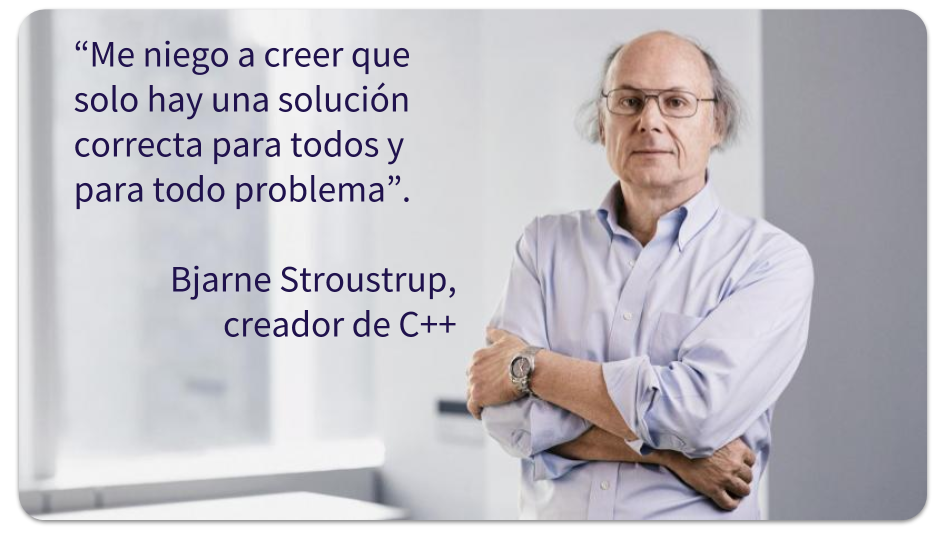
\includegraphics[width=1.0\textwidth]{CppIntro}
        \end{figure}


        % =========================================================
        % ==========          VENTAJAS DE C++        ==============
        % =========================================================
        \clearpage
        \section{Grandes ventajas de \Cpp}

            Hay muchas razones por las cuales \Cpp es uno de los lenguajes más usados en
            la modernidad en la programación competitiva (si no es que el más).

            Puedes escuchar un video muy bonito para mi sobre porque elegir este lenguaje:

            \Link{https://www.youtube.com/watch?v=JBjjnqG0BP8}{Bjarne Stroustrup: Why I Created \Cpp}

            \begin{figure}[h]
                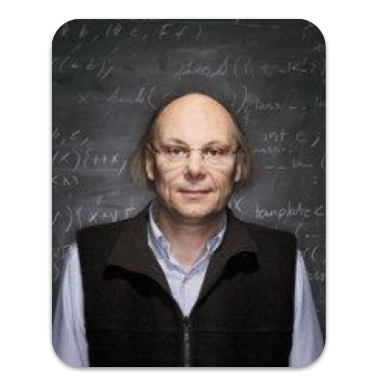
\includegraphics[width=0.35\textwidth]{BjarneBebe}
                \caption{\footnotesize{Este es el creador del lenguaje (reto: decir su nombre en voz alta) Bjarne Stroustrup}}
            \end{figure}


            Las principales razones por \Cpp sin un orden en particular son:
            \begin{itemize}
                \item \textbf{Te da abstracciones sin costo extra.}
                
                    O como lo diría su creador te da el poder de usar abstracciones de alto nivel pero sin que las mismas hagan tu programa
                    mas innecesariamente mas lento, o como lo dice la comunidad en inglés:

                    \begin{Indentation}[1.2em]
                    \Quote{
                        C++ has the zero-overhead principle: \textCode{what you don’t use, you don’t pay for}, that is,
                        with every new feature added to the language, you get at least as good performance as
                        if that feature will not be included.
                        
                        Also there are the principle:
                        \textCode{What you do use cost either only as much as what you’d implement yourself, or it cost less}, 
                        meaning that a new feature can either mantain or improve the performance.
                    }
                    \end{Indentation}
                
                    Personalmente creo que esa es mayor ventaja que tiene sobre todos los demás y que
                    resume perfectamente todo el objetivo de \Cpp.

                    Lo que nos dice esto es que podremos representar grafos, matrices, operaciones, 
                    clases en general, algoritmos, etc... en nuestros programas con gran facilidad,
                    cosa que no podemos hacer fácilmente por ejemplo en lenguajes como C o la familia
                    de los ensambladores.

                    \textit{
                    Y podrías decir, pero en Java o en Python podemos representar de una manera igual de fácil 
                    así que ... ¿porqué usar \Cpp?
                    }

                    Pues porque en todos los demás lenguajes estas pagando un costo (a veces muy grande de varios cientos 
                    o miles de veces) por poder representar ideas o conceptos abstractos en un programa, en \Cpp
                    esta prácticamente garantizado que usar una clase por ejemplo o que usar un arreglo que se auto
                    dimensiona (vector) no será más costoso que si lo hubieras hecho tu desde ensamblador.


                \item \textbf{Tienes a la biblioteca estandar, la gran std::* a tu lado}

                    Esta es otra gran ventaja, ya que siguiendo con la mentalidad de abstracciones sin costo extra tenemos
                    gracias a la gran libreria estándar un montón de cosas que no tenemos que hacer desde cero, desde
                    arreglos que cambian de tamaño, arreglos asociativos, pilas, colas, algoritmos de ordenamiento, 
                    de búsqueda, algoritmos para filtrar información, para hacer particiones o permutaciones, etc...

                    Así podemos dejar los algoritmos básicos al lenguaje y enfocarnos en las cosas que son de verdad interesantes.


                \item \textbf{Es \Quote{statically typed and compiled}, el compilador es tu amigo}

                    Otra ventaja más, podemos siempre confiar en el compilador, en que si nuestro programa compila muy probablemente
                    está haciendo lo que debe hacer (cosa que no podemos esperar con python por ejemplo), el compilador es tu amigo,
                    te dira en donde te equivocaste, en donde puede que hayas querido decir otra cosa y muchas veces te dará
                    consejos, además, tras bambalinas está transformando tu código en algo que la computadora puede de verdad
                    entender y además usará toda la información que le diste para muchas veces incluso mejorar tu código en vez
                    de solo \Quote{traducirlo} y optimizarlo de maneras que me sorprenden personalmente.


                \item \textbf{Es prácticamente un \Quote{super set} de C}
                
                    Es decir, que (casi) cualquier código válido de C es válido en \Cpp, esto es de gran ayuda pues
                    C es uno de los lenguajes más conocidos por lo que puede que la sintaxis de \Cpp sea
                    más fácil que entender la sintaxis de Haskell, de Kotlin o Prolog, por ejemplo. 
                    
                    Otra ventaja es que al estar basados en C conserva muchas de las ventajas de C como su portabilidad, 
                    su velocidad de ejecución  y la capacidad de tener un gran control de todos los recursos del sistema 
                    (memoria y tiempo de vida de un objecto, cough cough Java y su recolector de basura)

                \clearpage

                \item \textbf{Tienes un gran control de todos los recursos del sistema}
                
                    Esto es también es muy importante, pues nos dice que en \Cpp podemos controlar con gran lujo de detalle
                    los recursos del sistema, como por ejemplo la memoria.

                    \Cpp nos da el control de decidir por ejemplo a que lugar va cada variable (heap o al stack), 
                    lo cual es esencial para hacer un programa de alto rendimiento (y creeme que lo necesitaras).

                    \textbf{Es determinista.}

                    Es decir la limpieza de los objectos una vez que ya se acabaron de usar es solicitada cuanto tu quieres,
                    y no \textit{cuando el recolector de basura decide hacerlo}.

                    Tenemos el control de decidir si queremos pasar las cosas por referencia o por valor, si deseamos mover
                    un objecto o si una referencia no podrá ser modificada.

                \item {Tienes \textit{value types} por defecto (pero también tiene referencias si las necesitas)}.
                
                    Esta quiza sea algo rara de explicar si es que no conoces muchos sobre lenguajes de computación, y si
                    no la entiendes no te preocupes. 

                    Lo que nos dice es que las variables en \Cpp son variables de valor por defecto, es decir
                    cuando decimos \textCode{auto x = 10} nuestra variable \textCode{x} de verdad es el fragmento
                    de memoria que tiene ese 10.
                    
                    En otras palabras que nuestras variable de verdad almacenan la información que queremos \textbf{
                        y no una referencia que apunta a donde esta nuestra información
                    }.

                    Claro que aún puedes expresar la idea de las referencias, pero por defecto hablamos de variables que almacenan valores.
            \end{itemize}


        % =========================================================
        % ==========             VS OTROS            ==============
        % =========================================================
        \clearpage
        \section{\Cpp vs otros lenguajes}

            % ============================================
            % ========          VS C        ==============
            % ============================================
            \subsection{vs C}

                El gran problema con C es que es un lenguaje muy pequeño en el sentido en que todo lo tienes que hacer tu,
                si quieres hacer un problema que involucra cosas medio complejas todas las estructuras las tienes que codear
                al momento, y en un deporte de tiempo, cada segundo cuenta, así que en resumén, lo que \Quote{mata} a C es la falta
                de algo parecido a la std de \Cpp.

                Aunque para problemas sencillos C también puede ser una opción, (pero ya que $\Cpp$ es casi casi
                un superset de C podrías entonces igual de fácil hacerlo en $\Cpp$).

            % ============================================
            % ==========       VS JAVA          ==========
            % ============================================
            \subsection{vs Java}

                Con toda honestidad hay un porcentaje de la comunidad de programación competitiva que usan Java, así que
                si que es una opción viable, sobretodo por su gran libreria estándar y también porque en C++ no hay algo parecido
                a \textCode{BigInteger} y \textCode{BigDecimal} y suelen ser muchos los problemas que lo requieran, así que si bien \Cpp
                podría ser tu lenguaje por defecto es importante que también conozcas lo básico de Java (O Kotlin si quieres ser feliz).

            % ============================================
            % ==========        VS PYTHON        =========
            % ============================================
            \subsection{vs Python}

                Python es un gran lenguaje pero tiene todas las de perder en programción competitiva pues
                a ser interpretado y debilmente tipado, sus programas acaban siendo muy lentos incluso usando el 
                algoritmo correcto, eso si, hay varias aplicaciones útiles de Python, como que todos los
                enteros tienen infinita precisión por defecto (aka \textCode{BigInteger} como en Java).

                Así que tampoco es una mala idea aprenderlo por si se necesita un día, pero definitivamente
                no es la mejor idea para ser tu lenguaje por defecto en programación competitiva.


        % =========================================================
        % ==========          CPP MODERNO            ==============
        % =========================================================
        \clearpage
        \section{ Una pincelada de \Cpp moderno}

            Incluso en términos solo de sintaxis te perdonaría si pensaras que \Cpp es un
            lenguaje terminado, algo que se hizo en los 90's y que seguimos escribiendo
            igual al día de hoy.

            Y no es así, \Cpp 11 / 14 / 17 / 20 son cosas muy diferentes, igual de flexibles
            y de rápidas que el clásico \Cpp 98 pero mucho mas seguro y limpio de escribir.

            Mira un ejemplo.

            \begin{lstlisting}[language=C++, gobble=16]
                //Old C++
                circle* p = new circle(42);
                vector<shape*> v = load_shapes();

                for (vector<shape*>:::iterator i = v.begin(): i != v.end(); ++i) {
                    if (*i && **i == *p)
                        cout << **i << "is a match" << '\n';
                }

                // ...later, possible elsewhere

                for (vector<shape*>:::iterator i = v.begin(): i != v.end(); ++i) {
                    delete *i;
                }

                delete p;
            \end{lstlisting}

            Mientras que ahora podrías hacer algo como:
            \begin{lstlisting}[language=C++, gobble=16]
                //New badass C++
                auto p = make_shared<circle> (42);
                vector<shape*> v = load_shapes();

                for (auto& s : v) {
                    if (s && *s == *p)
                        cout << *s << "is a match" << '\n';
                }
            \end{lstlisting}

            \clearpage

            Veamos otro ejemplo, imagina que alguien te da una secuencia de 
            puntos (flotantes por ejemplo) y te pide calcular su media.

            Veamos como sería hacerlo en Python así de volada:
            \begin{lstlisting}[language=python, gobble=16]
                def mean(seq):
                    n = 0.0
                    for x in seq:
                        n += x
                    return n / len(seq)
            \end{lstlisting}

            Y en \Cpp mira como sería:
            \begin{lstlisting}[language=C++, gobble=16]
                auto mean(const Sequence& seq) {
                    auto n {0.0};
                    for (auto x : seq)
                        n += x;
                    return n / seq.size();
                }
            \end{lstlisting}

            Que bonito, ¿no?
            \cite{ModernCppWhatYouNeedToKnow}

    % ===============================================================================
    % ==========       Instalando y corriendo programas de C++          =============
    % ===============================================================================
    \clearpage
    \chapter{Instalando y corriendo programas de C++ y usar jueces}


    % ===============================================================================
    % ===============             BASES DEL LENGUAJE          =======================
    % ===============================================================================
    \clearpage
    \chapter{Bases del Lenguaje Moderno}

        \begin{wrapfigure}{r}{0.15\textwidth}
            \centering
            
\includegraphics[width=0.15\textwidth]{Warning}
        \end{wrapfigure}

        \textbf{
            Recuerda que esta sección del texto NO es una introducción a la programación para
            alguien que nunca ha programado nada en su vida, sino solo para alguien que
            no sabe \Cpp. 
        }

        \textbf{
            Si tu aún no sabes nada sobre como programar entonces recomiendo que busques un documento, tutorial, libro, etc...
            diseñado para empezar a programar, porque en este texto voy a dar varias cosas por sentado
            que deberían ser muy obvias para alguien que ya haya aprendido a programar, en cualquier
            lenguaje.
        }

        \textbf{
            Unas recomendaciones serían: 
            \begin{itemize}
                \item 
                    \underline{\href{https://platzi.com/cursos/programacion-basica/}
                    {Curso de programación básico de Platzi}}
                \item 
                    \underline{\href{https://youtu.be/duhDovqHbEs?list=WL}
                    {Every Programming Language in 15 Minutes - Brian Will}}
            \end{itemize}
        }

        \textbf{
            No te preocupes, te espero \textCode{<3}.
        }
        
        \textbf{
            Además si ya sabes \Cpp o no te interesa aprender toda la sintaxis e ir directo a cosas
            algo más relacionadas con la programación competitiva entonces puedes saltar hasta el
            siguiente capítulo dando click \underline{\hyperref[part:EstructurasDeDatos]{aquí}}.
        }



        % =========================================================
        % ========               VARIABLES           ==============
        % =========================================================
        \clearpage
        \section{Variables}

            En \Cpp (como en casi cualquier otro lenguaje) la idea obvia con la que podemos empezar
            es las variables, después de todo la programación siempre se trata sobre información (data) 
            y podemos ver a una variable como una unidad de información.

            En \Cpp una variable es un fragmento de memoria que almacena algun valor, 
            podemos tener variables que almacen lo que nosotros entenderemos, como números enteros
            o que almacenen cadenas o que almacenen una secuencia de racionales, etc...

            Como sabes en programación, tu eres el que elige el nombre de las variables y aunque puede
            ser lo que quieras, como \textCode{x, y, someNumber, patata} intenta elegir nombres que expresen
            lo que esta variable guardará como por ejemplo \textCode{numberOfDays, sizeOfSquare, words}. 

            Bueno, \Cpp es un lenguaje de tipado estatico (static typing), es decir que todo momento el compilador,
            para poder transformar tu programa a algo que una computadora pueda entender, tiene
            que saber que tipo de dato almacena esa variable.

            % ============================================
            % ====   DECLARACIONES E INICIALIZACION   ====
            % ============================================
            \subsection{Declaraciones e Inicialización}

                El primer paso para poder usar una variable será el de declararla, es decir
                aquí entre nos es decirle al compilador que le de a un fragmento de memoria 
                un nombre y que usaremos ese nombre (o identificador) para referirnos a ella después.

                La sintaxis es sencilla:
                \begin{lstlisting}[language=C++, gobble=20]
                    datatype variableName;

                    //Examples
                    int numberOfDays;
                    float pi;
                    bool isClosed;
                \end{lstlisting}

                Ahora, algo importante en \Cpp es que declarar una variable no la inicializa, 
                es decir, que al decir \textCode{int numberOfDays} nunca le estoy dando un valor a
                esa variable, por lo que ahora mismo la información que este guardada ahi es un misterio,
                es como si comprarás una bodega; solo por decir que es tuya no quiere decir que ahora este
                vacía.

                Por eso es tan poco común ver en la programación competitiva (y en la programación en general)
                declaraciones SIN inicializaciones,
                pues generan una gran cantidad de bugs que son difíciles de encontrar pues muchas veces
                por simple suerte la variable si se inicializa a un valor que tenga sentido, pero
                al ser este proceso aleatorio no es una gran idea depender de eso.

                \textbf{Además es una buena costumbre, no declarar variables hasta que tenga un valor coherente para
                las mismas}.

                \clearpage

                Muy unido a esto decimos que estamos inicializando una variable cuando le damos
                un valor por primera vez a este fragmento de la memoria.
                
                Puedes declarar variables en C++ de dos maneras:

                % ============================================
                % ======            SE DIRECTO          ======
                % ============================================
                \subsubsection{Se directo con el tipo de dato}

                    Algo como:
                    \begin{lstlisting}[language=C++, gobble=24]
                        int someNumber = 20;          //Good: declaration + initialization
                        string someText = "Hi baby";  //Good: declaration + initialization
                        double myLoveForYou;          //Bad: just declaration
                    \end{lstlisting}

                    Es decir, la sintaxis es:
                    \begin{itemize}
                        \item Primero el tipo de dato, después un espacio.
                        \item Después el nombre que le quieres dar a la variable.
                        \item Si quieres un valor inicial.
                    \end{itemize} 

                % ============================================
                % ======            SE SUTIL            ======
                % ============================================
                \subsubsection{auto: Se sútil}

                    Si es que es obvio que tipo de dato debería ser entonces puedes usar \textCode{auto}
                    que lo que nos dice es, compilador, yo se que eres un inteligente, anda, 
                    tu solito sabes de que tipo de dato es esta variable para que te lo repito yo.
                    
                    Y se hace hastante similar:
                    \begin{lstlisting}[language=C++, gobble=24]
                        auto someNumber = 20;        //someNumber is int
                        auto someText = "Hi baby";   //someText is const char* (this is sad)
                        auto myLoveForYou;           //This will not compile :v
                    \end{lstlisting}

                    Nota que para que puedas usar \textCode{auto} el compilador tiene que saber que tipo
                    de dato va a guardar esa variable así que si no inicializas la variable 
                    el compilador se va a enojar contigo.

                    De igual manera creo que te habras dado cuenta que podemos inicializar de dos maneras
                    generalmente la primera es muy obvia y en casi todos los lenguajes existe, se llama
                    \textbf{una asignación}, es decir, darle un valor a esa variable y se usa casi siempre en
                    todos los Lenguaje el símbolo \textCode{=} o a veces incluso \textCode{<-}.

                    Total, lo que pasa en \Cpp es que además de esa forma de inicializar variables tenemos
                    una forma que si tiene un nombre especial.

                % ============================================
                % ======            SE SUTIL            ======
                % ============================================
                \subsubsection{Uniform (brace) Inicialization: Inicialización uniforme}

                    Y lo que nos da esto es una misma sintaxis, quiza esto sea un tema algo complejo
                    para unos y no te preocupes si no entiendes esto por completo por ahora.

                    Total, lo que pasa es que en \Cpp moderno existe la sintaxis 
                    \textCode{type wea \{something\}} donde lo que hacemos es poner entre estas cosas
                    \textCode{ \{ \} } el valor con el que queremos inicializar nuestra variable y dependiendo
                    de que sea nuestra variable puedes simplemente asignarla o llamar al constructor con estos
                    parámetro.

                    Total, es solo una forma mas bonita de hacer las cosas.

                    \begin{lstlisting}[language=C++, gobble=24]
                        auto someNumber {20};   
                        string someText {"Hi baby"};
                        // this call a someClass constructor
                        someClass object {"some parameter", someNumber};
                        vector<int> numbers {1, 2, 3, 4, 5, 6};
                    \end{lstlisting}

                    Además ayuda en varias cosas:
                    \begin{itemize}
                        \item 
                            Supón que quieres inicializar por defecto un vector, entonces puedes hacer como:
                            \begin{lstlisting}[language=C++, gobble=28]
                                vector<int> days ();   
                            \end{lstlisting}

                            Expecto que esto es la declaración de una función llamada \textCode{days} que no 
                            recibe nada y regresa un vector.

                            En la antigüedad podríamos hacer algo como:
                            \begin{lstlisting}[language=C++, gobble=28]
                                vector<int> days = vector<int>();   
                            \end{lstlisting}

                            Pero ahora algo mucho mas sencillo gracias a uniform inicialization:
                            \begin{lstlisting}[language=C++, gobble=28]
                                vector<int> days {};   
                            \end{lstlisting}

                    \end{itemize}

        % =========================================================
        % ======         TIPOS DE DATOS NUMERICOS          ========
        % =========================================================
        \clearpage
        \section{Tipos de datos numéricos}

            % ============================================
            % ======     INTEGERS: ENTEROS          ======
            % ============================================
            \subsection{Integers / Integrals: Enteros}

                \Cpp (y C) maneja varios tamaños estándares de enteros, el más clásico
                es \textCode{int}, pero no es el único, los demás solo cambian en tamaño
                (y por los tanto los números que podemos almacenar)
                y estos son, de menor a mayor: \textCode{char, short, int, long y long long}.

                Así que con esto conocido, veamos las características más detalladamente de cada tipo:
                Pero si quieres un resumen, \Cpp garantiza que:
                \begin{lstlisting}[language=C++, gobble=20]
                    1 == sizeof(char) <= sizeof(short) <= sizeof(int) <= sizeof(long) <= sizeof(long long);
                \end{lstlisting}


                % ============================================
                % ==========        CHAR            ==========
                % ============================================
                \subsubsection{char}

                    A ver, técnicamente este tipo de dato como su nombre lo dice esta diseñado para almacenar
                    un carácter, lo que pasa es que en computación (no nos compliquemos la vida con UFT ahora)
                    un carácter como \textCode{'a'} ó \textCode{'p'} se representa internamente usando el código
                    ASCII (deberías buscar más de esto cuando tengas tiempo).
                    
                    Total, que en resumen este tipo de dato nació para almacenar un carácter de ASCII, 
                    por lo tanto es un tipo de datos numérico que va de 0 a 255.

                    No te preocupes si no entiendes las primeras líneas, pero si lo haces, muy bien por ti.
                    \begin{lstlisting}[language=C++, gobble=24]
                        auto character {'a'};                   // character is a char!
                        char number {23};                       // number is a char!

                        // Things that are true
                        ('a' == 97) and ('z' == 122);           // ASCII is just numbers
                        ('A' == 65) and ('Z' == 90);            // ASCII is just numbers
                        ('A' + 1 == 'B') and ('Z' - 1 == 'Y');  // You can do arithmetic

                        auto size {"char is 1 byte"};
                        char minValue {-128};
                        char maxValue {127};
                    \end{lstlisting}


                % ============================================
                % ==========        INT            ===========
                % ============================================
                \clearpage
                \subsubsection{int}

                    Es el tipo de dato numérico estándar en \Cpp, así que si declaras un número
                    con \textCode{auto} entonces lo más probable es que sea \textCode{int}.

                    Ahora, pasa algo raro con este tipo de dato, que dependiendo de la máquina
                    en la que compiles entonces puede tener 2 o 4 bytes de tamaño (usa el que
                    sea más eficiente para el sistema), aun así, casi nunca compilaras en 
                    algún sistema que te diga que un \textCode{int} es de 2 bytes, así que para
                    este texto usaremos que \textCode{int} es de 4 bytes.
                    \begin{lstlisting}[language=C++, gobble=24]
                        auto number {23};                           // number is an int!

                        auto size {"int is 4 bytes"};
                        int minValue {-2,147,483,648};
                        int maxValue {2,147,483,647};
                    \end{lstlisting}

                % ============================================
                % ==========        LONG           ===========
                % ============================================
                \subsubsection{long long}

                    Este no es un tipo de dato, per se, sino que es un modificador que le puedes aplicar
                    a \textCode{int} y con esto lo que logras es crear un tipo de dato que tiene al menos 8 bytes.

                    Por eso es que ignore a \textCode{long int / long} pues solo nos garantiza que tendra al menos 4 bytes
                    por lo que es mas o menos inútil, lo mas seguro es declarar algo como \textCode{long long}
                    si te interesa que tenga el máximo tamaño posible.
                    \begin{lstlisting}[language=C++, gobble=24]
                        int normalVariable {};                      // It takes 4 bytes     
                        long long int normalVariable {};            // It takes 8 bytes 
                        auto number {1,000,000,000,000,000,000}     // number is long long  

                        auto size {"long long int is 8 bytes"};
                        long long minValue {-9,223,372,036,854,775,808};
                        long long maxValue {9,223,372,036,854,775,807};
                    \end{lstlisting}


                % ============================================
                % ==========        UNSIGNED       ===========
                % ============================================
                \subsubsection{unsigned}

                    Lo que hace este modificador (exacto, esto tampoco es un tipo de dato)
                    es eliminar el signo de los tipos numéricos, es decir el entero más bajo que vas
                    a poder guardar va a ser el 0, pero con ello vas a lograr duplicar
                    el máximo entero que puedes almacenar y no aumentas para nada el espacio necesario :o
                    \begin{lstlisting}[language=C++, gobble=24]
                        char maxValueChar {127};                    
                        unsigned char maxValueIntUnsigned {255};
                        
                        int maxValueInt {2,147,483,647};                    
                        unsigned int maxValueIntUnsigned {4,294,967,295};
                        
                        long long maxValueLL {9,223,372,036,854,775,807};                    
                        unsigned long long maxValueLLUnsigned {18,446,744,073,709,551,615};
                    \end{lstlisting}


                % ============================================
                % ==========        UNSIGNED       ===========
                % ============================================
                \subsubsection{short}

                    Hace lo inverso que \textCode{long}, en vez que duplicar el tamaño lo parte a la mitad,
                    y ya, solo eso :v

                    \begin{lstlisting}[language=C++, gobble=24]
                        auto size {"short is 2 bytes"};
                        short int minValue {-32,768};
                        short int maxValue {32,767};
                    \end{lstlisting}
                
                % ============================================
                % ==========        SIZE_T         ===========
                % ============================================
                \subsubsection{std::size\_t}

                    Este es especial y muchas veces lo usaré como estándar de tipo numérico
                    y es que usamos muchas veces los enteros como índice de un contenedor.

                    Bien pues \textCode{size\_t} es un tipo de dato especial que nos da \Cpp
                    que nos asegura que será tan grande como necesitemos para usarlo como índice
                    de cualquier contenedor.

                    Nota que como lo usamos para índice, este tipo de dato no tiene signo y generalmente tiene
                    el mismo tamaño de que un \textCode{long long}.

                    Además si te gusta los detalles visita esto:
                    \underline{\href{https://stackoverflow.com/questions/4849678/c-for-loop-size-type-vs-size-t}{aquí}}.

                    Por ejemplo, \textCode{std::vector, std::string, std::array} y más lo usan
                    como índice.
                    \begin{lstlisting}[language=C++, gobble=24]
                        std::vector<int> someIntegers {1, 2, 3, 4, 20, 5};
                        std::size_t numberOfElements {someIntegers.size()}; 
                    \end{lstlisting}


                % ============================================
                % ==========        FIXED WIDTH     ==========
                % ============================================
                \subsubsection{Fixed width (int32\_t, uint64\_t, ...)}

                Si prefieres estar seguro del tamaño de tus enteros entonces puedes usar 
                \textCode{\#include <cstdint>} que no incluye otros tipos de datos diferentes sino solo
                nos da alias (typedef / using), es decir otros nombres para los tipos de datos que ya conoces:
                \begin{lstlisting}[language=C++, gobble=20]
                    #include <cstdint>
                    
                    int8_t likeChar {};
                    int16_t likeShort {};
                    int32_t likeInt {};
                    int64_t likeLong {};

                    // And the unsigned versions:
                    uint8_t likeChar {};
                    uint16_t likeShort {};
                    uint32_t likeInt {};
                    uint64_t likeLong {};
                \end{lstlisting}
                    

            % ============================================
            % ====  FLOATING POINTS: PUNTO FLOTANTES  ====
            % ============================================
            \clearpage
            \subsection{Floating Points: Puntos Flotantes}

                A primera vista, los números de punto flotante parecen simples.
                Son solo enteros con puntos decimales, ¿verdad? 
                ¿Por qué no los usamos todo el tiempo, ya que pueden almacenar una mayor variedad de números?

                La respuesta es sencilla, no son precisos.

                \begin{figure}[h]
                    \centering
                    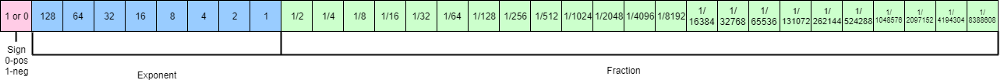
\includegraphics[width=0.9\textwidth]{IEEEFP}
                    \caption{\footnotesize{Representación del \textCode{float} en \Cpp}}
                \end{figure}

                Y ya, solo por eso, intenta poner en Python o en \Cpp si quieres esto 
                \textCode{(0.1 + 0.2) == 0.3} y verás que es falso, la razón es que los números de punto
                flotante tienen una cantidad límitada de dígitos de presición.

                Así que esta bien usarlos y todo, pero porfavor, hazlo con cuidado.

                Además así como \textCode{long long} era el doble que \textCode{int}, así
                \textCode{double} tiene el doble de presición (de ahí el nombre :v) que el clásico
                tipo de dato de punto flotante en \Cpp, \textCode{float}.

                \begin{lstlisting}[language=C++, gobble=20]
                    float almostPI {3.1};
                    double almostAlmostPI {3.14156};
                \end{lstlisting}
                

            % ============================================
            % =====  COMPLEX: NUMEROS COMPLEJOS     ======
            % ============================================
            \subsection{Complex: Números Complejos}

                Esta sección igual será corta, lo único que quiero decirte por si un día lo ocupas
                es que \Cpp tiene una clase que nos permite representar a los complejos.

                Nunca lo he ocupado de manera personal y no creo que sea el momento, en un texto introductorio
                de \Cpp, pero si un día lo necesitas, recuerda que \Cpp ya lo tiene integrado.

            
        % =========================================================
        % ======           OTROS TIPOS DE DATOS            ========
        % =========================================================
        \clearpage
        \section{Los otros tipos de datos fundamentales}

            % ============================================
            % ======             VOID               ======
            % ============================================
            \subsection{void}

                Este es bastante sencillo, (si no cuentas \textCode{*void}), y simplemente indica
                un tipo de dato vacío, es usado para mostrar que una función no regresa nada.
               
                Decimos que \textCode{void} tiene un conjunto vacío de elementos, es decir no puedes hacer
                variables (o instanciar) cosas de tipo  \textCode{void} por lo que muchas veces
                se le llama un tipo de dato incompleto.
                \begin{lstlisting}[language=C++, gobble=20]
                    void someVariable;  // Illegal
                \end{lstlisting}

            % ============================================
            % ======             BOOL               ======
            % ============================================
            \subsection{bool}

                Solo puede tener dos posibles valores, verdadero o falso, se llama así por el álgebra
                booleana, que justamente solo contaba con dos valores.
                \begin{lstlisting}[language=C++, gobble=20]
                    bool isSunny {true};
                    bool iAmHappy {false};
                \end{lstlisting}

                % ============================================
                % ======             BOOL               ======
                % ============================================
                \subsubsection{Cambiar el valor de un bool}

                    Como un \textCode{bool} solo puede tener un valor muchas veces queremos andar volteando
                    los valores de un valor booleano, es decir, primero eres \textCode{true}, luego
                    \textCode{false}, luego \textCode{true}, luego \textCode{false}, luego \textCode{true}, 
                    etc...

                    Para hacerlo lo que hacemos sera negar el antiguo valor que tenian y guardar ese nuevo valor,
                    esto se hara con algo como:
                    \begin{lstlisting}[language=C++, gobble=24]
                        bool isEven {true};
                        int n {};
                        while (true) {
                            cout << n << " " << isEven << '\n';
                            isEven = not isEven;        // The important line
                        }
                    \end{lstlisting}


        % =========================================================
        % ==========             OPERADORES              ==========
        % =========================================================
        \clearpage
        \section{Operadores}

            % ============================================
            % =====      OPERADORES ARITMETICOS     ======
            % ============================================
            \subsection{Operadores Aritméticos}

                Sección corta, si sabes programar los has usado:

                \begin{itemize}
                    \item \textCode{+}: Suma
                    \item \textCode{-}: Resta
                    \item \textCode{*}: Multiplicación
                \end{itemize}

                Además en C++ tenemos algunas ayudas para escribir menos:
                \begin{itemize}
                    \item \textCode{a++} es lo mismo que \textCode{a = a + 1}, ademas 
                        decimos que es una expresión regresa a \textCode{a} antes de hacer la suma.
                        \begin{lstlisting}[language=C++, gobble=28]
                            int a {1};
                            int b {a++};    // b is 1
                        \end{lstlisting}
                    \item \textCode{a---} es lo mismo que \textCode{a = a - 1} y con las mismas reglas que \textCode{a++}
                    \item \textCode{++a} es lo mismo que \textCode{a = a + 1}, ademas 
                        decimos que es una expresión regresa a \textCode{a} después de hacer la suma.
                        \begin{lstlisting}[language=C++, gobble=28]
                            int a {1};
                            int b {++a};    // b is 2
                        \end{lstlisting}
                    \item \textCode{a += b} es lo mismo que \textCode{a = a + b}
                    \item \textCode{a -= b} es lo mismo que \textCode{a = a - b}
                    \item \textCode{a *= b} es lo mismo que \textCode{a = a * b}
                    \item \dots
                \end{itemize}

                Ahora los interesantes son los siguientes:

            % ============================================
            % =====         DIVISION ENTERA         ======
            % ============================================
            \subsection{División entera}

                Una cosa que a mucha gente le cuesta es la división y no porque
                sea una operación difícil sino porque en \Cpp dependiendo de los
                valores a los que se la apliquemos se comportara de manera o de otra,
                si es que ambos valores son punto flotante entonces hara lo que esperas
                por ejemplo \textCode{1.0 / 2.0 = 0.5}, pero \textCode{1 / 2 != 0.5} porque
                si aplicas la división a dos enteros entonces hara la división entera, es decir
                va a redondeo al entero proximo mas pequeño.

                Hay que tener cuidado con eso.

            % ============================================
            % =====              MODULO             ======
            % ============================================
            \subsection{Lo que hay que saber del módulo: \textCode{\%}}
            
                El módulo es pocas palabras es el residuo de la división.

                Es decir \textCode{a \% b} regresa el residuo de la división $\dfrac{a}{b}$
                si la has visto entonces verás que es la misma que en todos los lenguajes
                sino entonces mas vale que practiques con unos ejemplos, es todo cuestión
                de practica.

                % ============================================
                % =====              MODULO             ======
                % ============================================
                \subsubsection{La respuesta para los puristas}

                    Si eres matemático y quieres la definición formal podríamos pensar en:

                    \begin{MultiLineEquation*}{3}
                        a \% b = a - floor(a / b) \; * \; b
                    \end{MultiLineEquation*}

                    Otra forma de verlos es que nos regresa un número \textCode{k}
                    tal que $k \equiv a \; \mod b$

                % ============================================
                % =====              EJEMPLOS           ======
                % ============================================
                \subsubsection{Ejemplos}
                
                    \begin{itemize}
                        \item $7 \% 5 = 2$
                        \item $5 \% 7 = 5$
                        \item $3 \% 7 = 3$
                        \item $2 \% 7 = 2$
                        \item $1 \% 7 = 1$
                    \end{itemize}

                    La forma mas común para lo que lo usamos
                    es para saber si un número es par o impar, donde
                    si $n$ es par entonces \textCode{n \% 2 == 0} y si es impar
                    entonces \textCode{n \% 2 == 1}.

                    En general, si quieres saber si un número $n$ es multiplo de 
                    otro $k$ entonces hay que checar que \textCode{n \% k == 0}.

            % ============================================
            % =====   OPERADORES RELACIONALES       ======
            % ============================================
            \clearpage
            \subsection{Operadores Relacionales}

                Estos sirven para comparar los elementos, también son practicamente iguales a como son en todos los
                lenguajes:
                \begin{itemize}
                    \item Igualdad Lógica: 
                    
                        Se escribe así y solo el valor de verdad de ambos valores es igual.
                        \begin{lstlisting}[language=C++, gobble=28]
                            bool IAmHappy = IHaveLove == true
                        \end{lstlisting}
                    
                    \item Desigualdad Lógica: 
                    
                        Se escribe así y solo el valor de verdad de ambos valores es diferente.
                        \begin{lstlisting}[language=C++, gobble=28]
                            bool IAmHappy = IHaveLove != true
                            bool IAmHappy = IHaveLove not_eq true
                        \end{lstlisting}

                    \item Mayor y menor: 
                        \begin{lstlisting}[language=C++, gobble=28]
                            int debt{20}, money{50};
                            bool IAmHappy = debt < money;
                            bool IAmHappy = money > debt;
                        \end{lstlisting}

                    \item Mayor / menor o igual: 
                        \begin{lstlisting}[language=C++, gobble=28]
                            int debt{20}, money{50};
                            bool IAmHappy = debt <= money;
                            bool IAmHappy = money >= debt;
                        \end{lstlisting}
                \end{itemize}


            % ============================================
            % =====       OPERADORES LOGICOS        ======
            % ============================================
            \subsection{Operadores Lógicos}

                En \Cpp tenemos varios operadores lógicos que tomaran como argumentos dos 
                \textCode{bool} o cosas que se puedan convertir a bool y con ellas nos darán otro
                valor booleano.

                \begin{itemize}
                    \item AND Lógico: 
                    
                        Se escribe así y solo será verdad si es que ambos parámetros son \textCode{true}.
                        \begin{lstlisting}[language=C++, gobble=28]
                            bool IAmHappy = IHaveAJob && IHaveAFreeTime 
                            bool IAmHappy = IHaveAJob and IHaveAFreeTime
                        \end{lstlisting}

                    \item OR Lógico: 
                    
                        Se escribe así y solo será verdad si es que al menos uno de los parámetros son \textCode{true}.
                        \begin{lstlisting}[language=C++, gobble=28]
                            bool IAmOk = IHaveAJob || IHaveAFreeTime 
                            bool IAmOk = IHaveAJob or IHaveAFreeTime
                        \end{lstlisting}

                    \item NOT Lógico: 
                    
                        Se escribe así y solo invierte el valor de verdad de lo que le enviemos.
                        \begin{lstlisting}[language=C++, gobble=28]
                            bool IAmHappy = !IAmSad
                            bool IAmHappy = not IAmSad
                        \end{lstlisting}

                \end{itemize}


            % ============================================
            % =====       OPERADORES LOGICOS        ======
            % ============================================
            \subsection{Operadores Lógicos bit a bit}

                En \Cpp tenemos varios operadores lógicos bit a bit que tomaran como argumentos dos números 
                y nos regresan otro numero.

                Ahora, los demás operadores son tan obvios que practicamente no tengo nada que decir, pero para estos si que tengo
                mucho que decir, y antes de que diga mas hay que recordar el binario, y como funciona, 
                asi que si algo te suena raro recuerda checar si estas entendiendo bien el binario, ahora si, 
                veamoslos con cuidado:

                \begin{itemize}
                    \item AND Lógico bit a bit: 
                    
                        Se escribe así, y lo que hace es aplicar AND bit a bit de nuestros números, es decir
                        un bit es 1 si y solo si es que ambos son 1.
                        \begin{lstlisting}[language=C++, gobble=32]
                            int number1 {0b11100011};   // C++14
                            int number2 {0b01010101};   // C++14

                            int numberAND = number1 & number2;
                            int numberAND = number1 bitand number2;
                        \end{lstlisting}

                        Donde tendremos que \textCode{numberAND = 0b01000001}. Mira porque:
                        \begin{lstlisting}[language=C++, gobble=32]
                            11100011    -> number1
                            & 01010101    -> number2
                            ---------
                            01000001
                        \end{lstlisting}
                        
                    \item OR Lógico bit a bit: 
                    
                        Explicado el AND logico, este es basicamente el mismo, pero que ahora siguiendo el OR, es
                        decir, solo si alguno de los dos es uno entonces el valor de ese bit será uno.
                        \begin{lstlisting}[language=C++, gobble=32]
                            int number1 {0b11100011};   // C++14
                            int number2 {0b01010101};   // C++14

                            int numberOR = number1 | number2;
                            int numberOR = number1 bitor number2;
                        \end{lstlisting}

                        Donde tendremos que \textCode{numberOR = 0b11110111}. Mira porque:
                        \begin{lstlisting}[language=C++, gobble=32]
                            11100011    -> number1
                            & 01010101    -> number2
                            ---------
                            11110111
                        \end{lstlisting}
                    
                    \item XOR Lógico bit a bit: 
                    
                        Lo mismo pero siguiendo ahora el XOR bit a bit:
                        \begin{lstlisting}[language=C++, gobble=32]
                            int number1 {0b11100011};   // C++14
                            int number2 {0b01010101};   // C++14

                            int numberXOR = number1 ^ number2;
                            int numberXOR = number1 xor number2;
                        \end{lstlisting}

                        Donde tendremos que \textCode{numberXOR = 0b10110110}. Mira porque:
                        \begin{lstlisting}[language=C++, gobble=32]
                            11100011    -> number1
                            & 01010101    -> number2
                            ---------
                            10110110
                        \end{lstlisting}

                    \item Negación Lógica bit a bit: 
                    
                        Lo que hace es negar cada bit:
                        \begin{lstlisting}[language=C++, gobble=32]
                            int number {0b11100011};   // C++14
                            int numberNeg = ~number;
                            int numberNeg = compl number;
                        \end{lstlisting}

                        Donde tendremos que \textCode{numberNeg = 0b00011100}. Mira porque:
                        \begin{lstlisting}[language=C++, gobble=32]
                            11100011    -> number
                            ---------
                            00011100
                        \end{lstlisting}
                    
                    \item Shifts bit a bit:
                    
                        Toma dos números y lo que hace es desplazar el primer número la cantidad que dice el 
                        segundo número de veces y llena lo que va moviendo con 0's, 
                        veamos las dos versiones que tenemos: 
                        \begin{itemize}
                            \item Left shift
                                \begin{lstlisting}[language=C++, gobble=40]
                                    int number {0b00000110};
                                    int number1 = number << 1;      // 0b00001100
                                    int number2 = number << 3;      // 0b00110000
                                \end{lstlisting}

                            \item right shift
                                \begin{lstlisting}[language=C++, gobble=40]
                                    int number {0b00000110};
                                    int number1 = number >> 1;      // 0b00000011
                                    int number2 = number >> 2;      // 0b00000001
                                    int number3 = number >> 3;      // 0b00000000
                                \end{lstlisting}

                        \end{itemize}
                    
                \end{itemize}



        % =========================================================
        % ==========        SENTENCIAS DE CONTROL        ==========
        % =========================================================
        \clearpage
        \section{Sentencias de Control}

            % ============================================
            % =======        CONDICIONALES         =======
            % ============================================
            \subsection{Branching: Condicionales}

                Sin una declaración de un condicional como la instrucción \textCode{if}, los programas
                se ejecutarian siempre de la misma manera.
                
                Los condicionales permiten que se cambie el flujo del programa y con ello códigos
                más interesantes.

                \begin{lstlisting}[language=C++, gobble=20]
                    //Simpler form
                    if (condition) {
                        ...
                    }

                    //Simple form
                    if (condition) {
                        ...
                    }
                    else {
                        ...
                    }
                    
                    //Complete form
                    if (condition1) {
                        ...
                    }
                    else if (condition2) {
                        ...
                    }
                    else if (condition3) {
                        ...
                    }
                    else {
                        ...
                    }
                \end{lstlisting}


                % ============================================
                % =======        CONDICIONES           =======
                % ============================================
                \clearpage
                \subsubsection{Condiciones}

                En \Cpp lo que puede ir dentro del \textCode{if (condition)} pueden ser dos cosas:
                \begin{itemize}
                    \item Una expresión que se pueda transformar a un \textCode{bool} y eso es la cosa
                        mas común.

                        Por ejemplo:
                        \begin{lstlisting}[language=C++, gobble=28]
                            bool isSunny {true};
                            if (isSunny == true) {
                                cout << "Hey, time to go to outside" << '\n';
                            }

                            if (isSunny) {
                                cout << "Hey, it is the same but shorter syntax" << '\n';
                            }

                            double pi {3.1416}, e {2.71828};
                            if (pi > e) {
                                cout << "Math still make sense" << '\n';
                            }
                        \end{lstlisting}

                        Tambien podemos poner dentro del if una variable lo que hara
                        que \Cpp transforme el valor de dicha variable en un booleano,
                        las reglas que sigue son bastante sencillas:
                        \begin{lstlisting}[language=C++, gobble=28]
                            if (n) {
                                ...
                            }
                        \end{lstlisting}
                        \begin{itemize}
                            \item Para números: Si n es cero entonces el if evaluara a falso, para
                                cualquier otro valor será verdadero. 
                            \item Para strings: Si n esa vacío entonces sera falso, cualquier otra
                                otro valor será verdadero. 
                            \item Para punteros: Si n es NULL / nullptr entonces sera falso, cualquier otra
                                otro valor será verdadero. 
                        \end{itemize}

                    \item Se puede hacer \textCode{if (a = b)} en cuyo caso lo que comparará el 
                        \textCode{if} es el resultado de la asignación.
                \end{itemize}

                % ============================================
                % =======        OPERADOR TERNARIO     =======
                % ============================================
                \clearpage
                \subsubsection{Operador Ternario}

                En \Cpp tenemos el operador ternario, es bastante común porque nos deja expresar la misma
                idea que un \textCode{if} pero mucho mas corto, además es una expresión, es decir
                regresa un valor, esa es la más grande referencia.

                Y por lo tanto es muy útil cuando lo único que hacemos es darle un valor a una variable
                o algo relativamente sencillo.

                \begin{lstlisting}[language=C++, gobble=20]
                    // Using if else
                    auto programmerFeelings = "";
                    if (language == "php") {
                        programmerFeelings = "sad";
                    }
                    else {
                        programmerFeelings = "happy";
                    }

                    // The same thing using ternary operator
                    auto programmerFeelings = (language == "php") ? "sad" : "happy";
                \end{lstlisting}
                
        % =========================================================
        % ==========               CICLOS                ==========
        % =========================================================
        \clearpage
        \section{Ciclos}
            
            En \Cpp tenemos distintos tipos de ciclos, y si funcionan exactamente igual que
            en todos los demás lenguajes, tenemos:

            
            % ============================================
            % =======           WHILE              =======
            % ============================================
            \subsection{While}

                \begin{lstlisting}[language=C++, gobble=20]
                    while (condition) {
                        // statements
                    }
                \end{lstlisting}

                Donde condition es exactamente igual que lo que estaría dentro
                del if.

                Y de hecho funciona basicamente igual que un if, la única diferencia
                es que una vez que se haya ejecutado el cuerpo entonces volveremos a ver la 
                condición, de ser verdadera el cuerpo se volverá a ejecutar.

                % ============================================
                % =======          DO WHILE            =======
                % ============================================
                \subsubsection{Do while}

                    Existe también una variante que se llamada \textCode{do while} y que 
                    es bastante menos conocido que el clásico \textCode{while}, así que creo
                    que vale la pena hablar un poco de el.

                    \begin{lstlisting}[language=C++, gobble=24]
                        do {
                            // statements
                        }
                        while (condition);
                    \end{lstlisting}

                    En este ciclo primero ejecutamos las instrucciones que esten dentro del bloque
                    y luego es que checamos la condición y si es verdadera entonces volvemos 
                    ejecutar las instrucciones.

            % ============================================
            % =======           FOR                =======
            % ============================================
            \clearpage
            \subsection{For}

                Igual que en cualquier otro lenguaje:
                \begin{lstlisting}[language=C++, gobble=20]
                    for (init expr; condition expr; step expr) {
                        // statements
                    }
                \end{lstlisting}

                Que como sabes si sabes programar es exactamente igual que:
                \begin{lstlisting}[language=C++, gobble=20]
                    init expr;
                    while (condition expr) {
                        // statements
                        step expr;
                    }
                \end{lstlisting}

                Ahora, hablemos del nuevo pequeño ciclo en el lenguaje:

            % ============================================
            % =======           FOR                =======
            % ============================================
            \subsection{Range for: \textCode{for (auto x : v)}}

                En \Cpp tenemos otra forma más moderna y muchos diran que mucho mas
                fácil de evitar bugs raros si lo único que haremos será movernos un 
                elemento a la vez a lo largo de un contenedor, y si en efecto vamos a visitar cada
                elemento desde el inicio hasta el final del contendedor (no te preocupes, pronto
                hablaremos sobre contenedores) entonces puedes hacer un clásico:
                \begin{lstlisting}[language=C++, gobble=20]
                    for (type element : container) {
                        // statements
                    }
                \end{lstlisting}

                Por ejemplo:
                \begin{lstlisting}[language=C++, gobble=20]
                    vector<int> someNumbers {1, 2, 3, 4};

                    for (int i : someNumbers) {
                        cout << i << '\n';
                    }
                \end{lstlisting}

                Y si lo que quieres es iterar sobre elementos que pueden ser caros de copiar entonces
                podemos también usar una referencia (si no sabes que son, no te preocupes, pronto hablaremos de eso)
                de este y tener algo como:
                \begin{lstlisting}[language=C++, gobble=20]
                    vector<string> countryCodes {"USA", "MEX", "JAN", "UK", "CHL", "SA"};

                    for (string& countryCode : countryCodes) {
                        cout << countryCode << '\n';
                    }
                \end{lstlisting}

                Tambien sirve si es que quieres alterar los elementos del contenedor:
                \begin{lstlisting}[language=C++, gobble=20]
                    vector<int> numbers {1, 2, 3, 4};

                    for (int& number : numbers) {
                        number *= 3;
                    }

                    // Now numbers is [3, 6, 9, 12]
                \end{lstlisting}

                Y si, hablaremos sobre referencias y \textCode{auto\&\&} más a detalle pronto.


                Además puedes usar \textCode{break, continue} como en cualquier \textCode{for} normal
                \begin{lstlisting}[language=C++, gobble=20]
                    vector<int> numbers {1, 2, 3, 4};

                    for (int& number : numbers) {
                        if (number == 3) break;
                    }

                    for (int& number : numbers) {
                        if (number != 3) continue;
                        else {
                            ...
                        }
                    }
                \end{lstlisting}
        
        % =========================================================
        % ====  REFERENCES AND VALUES:  APUNTADORES Y VALORES  ====
        % =========================================================
        \clearpage
        \section{References and value types}

            % ============================================
            % ====  VALUE TYPES: VARIABLES DE VALOR  =====
            % ============================================
            \subsection{Value types: Variables de valor}

                En \Cpp como llevamos diciendo todo el libro las variables por defecto son de tipo
                valor, es decir que cada variable almanena de verdad sus valores.

                \begin{lstlisting}[language=C++, gobble=20]
                    int someNumber {3};
                \end{lstlisting}

                Pero no solo podemos expresar esa idea, sino que también podemos expresar la idea
                de una \Quote{referencia a una variable}. 


            % ============================================
            % =====    REFERENCIAS: REFERENCIAS     ======
            % ============================================
            \subsection{References: Referencias}

                Las referencias solo son otro nombre para una variable, es como un alias.

                Se usan cuando uno quiere estar pasando el valor de una variable sin tener que copiar la misma
                variable, recuerda: No es gran cosa copiar una pequeña variable, pero
                copiar contenedores (como vectores, arreglos, strings, etc...)
                pueden ralentizar mucho un programa.

                Además si sabes de C y sus punteros, entonces te puedo decir que las referencias
                cumplen una función parecida, pero también hacen el código más sencillo de leer
                al evitar cosas como los operadores de indirección: \textCode{*} y el operador flecha
                \textCode{->}.

                Una referencia se crea así:
                \begin{lstlisting}[language=C++, gobble=20]
                    int number {};
                    int& referenceToNumber {number};
                \end{lstlisting}

                \textbf{Ahora, una variable de tipo referencia esta unida desde el momento en el que se crea a otra.
                No puedes hacer que una variable de tipo referencia ahora haga referencia a otra variable después
                de ser creada, además una referencia siempre tiene que referir a una variable, no puede referir a
                la nada.}

                \clearpage

                Las referencias vienen a solucionar dos problemas bastante clasicos en programación, 
                sobretodo en \Cpp:
                \begin{itemize}
                    \item Hacer que las funciones afecten los argumentos que les pasas y no a copias
                        
                        Veamos un ejemplo, supongamos esta función:
                        \begin{lstlisting}[language=C++, gobble=28]
                            void add_3_to_this_number(int number) {
                                number += 3;
                            }
                        \end{lstlisting}

                        Entonces si hacemos algo como esto, ¿Qué esperas que pase?
                        \begin{lstlisting}[language=C++, gobble=28]
                            int the_number {0};
                            cout << the_number << '\n';       // prints 0
                            add_3_to_this_number(the_number);
                            cout << the_number << '\n';       // prints 0 :c
                        \end{lstlisting}

                        Si conoces como funcionan las funciones en \Cpp entonces es claro que
                        \textCode{the\_number} sigue valiendo 0, porque cuando usas una función,
                        estas de verdad creando una copia y es a esa copia a la que estas añadiendole 3.

                        Si quieres crear una función que de verdad tome a un entero y le sume 3 a ESE entero,
                        entonces podemos hacer que reciba el parámetro por referencia:
                        \begin{lstlisting}[language=C++, gobble=28]
                            void add_3_to_this_number(int& number) {
                                number += 3;
                            }

                            // later ...
                            
                            int the_number {0};
                            cout << the_number << '\n';       // prints 0
                            add_3_to_this_number(the_number);
                            cout << the_number << '\n';       // prints 3 :)
                        \end{lstlisting}

                    \item Evitar generar copias a lo estúpido:
                    
                        Encontre este texto en internet y no pude evitar compartirlo:

                        \Quote{
                            \textCode{You live in a house on a street in a town somewhere. 
                            I want to visit you to give you something.}

                            \textCode{I have two choices - you can tell me your address, 
                            and I’ll come to you, or you can bring your house on
                            the back of a huge truck to me. One of these is obviously ridiculous.}
                        }

                        O en español:

                        \Quote{
                            \textCode{Tu vives es una casa, en una calle cualquiera en algún pueblo.
                            Supón que te quiero visitar para darte algo.}

                            \textCode{Tienes dos opciones - me puedes decir tu dirección y yo ire contigo o
                            puedes traer tu casa en un camión enorme hasta mi.
                            Una de ellas es obviamente ridícula.}
                        }
                        \cite{RandomReference_Refeence1}
                        
                        Veamos otro ejemplo, supongamos esta función:
                        \begin{lstlisting}[language=C++, gobble=28]
                            int sumTheFirstTwoElements(vector<int> numbers) {
                                int result = numbers[0] + numbers[1];
                                return result;
                            }
                        \end{lstlisting}

                        Ahora, a diferencia del ejemplo de arriba no importa si es que \textCode{numbers}
                        es el vector en si o una copia, pero si es que estamos generando una copia entonces
                        estamos haciendo nuestro código mucho mas lento sin razón.

                        Ahora, podemos solucionar esto de manera muy sencilla como:
                        \begin{lstlisting}[language=C++, gobble=28]
                            int sumTheFirstTwoElements(vector<int>& numbers) {
                                int result = numbers[0] + numbers[1];
                                return result;
                            }
                        \end{lstlisting}

                        Ahora, si tienes miedo de pasar cosas por referencias por el miedo a que la 
                        función modifique tu argumentos entonces podemos hacer algo tan sencillo como:
                        \begin{lstlisting}[language=C++, gobble=28]
                            int sumTheFirstTwoElements(const vector<int>& numbers) {
                                int result = numbers[0] + numbers[1];
                                return result;
                            }
                        \end{lstlisting}
                        
                \end{itemize}

                % ============================================
                % =====    REFERENCES VS POINTERS       ======
                % ============================================
                \clearpage
                \subsubsection{References vs Pointer: Referencias vs Punteros}

                \begin{itemize}
                    \item Te evita problemas con \textCode{nullptr} / \textCode{NULL}:

                        Ve la siguiente función:
                        \begin{lstlisting}[language=C++, gobble=28]
                            int foo(bar* b1, bar* b2) {
                                return b1->calculate(b1->get());
                            }
                        \end{lstlisting}

                        Ahora, nada evita que pueda llamar a la función con algo como:
                        \begin{lstlisting}[language=C++, gobble=28]
                            int result = foo(NULL, NULL);       // If you like C
                            int result {foo(nullptr, nullptr)}; // If you like C++
                        \end{lstlisting}

                        Y el compilador no te dira nada, pero si hago algo como lo siguiente puedo solucionar el
                        problema:
                        \begin{lstlisting}[language=C++, gobble=28]
                            int foo2(const bar& b1, const bar& b2) {
                                return b1.calculate(b1.get());
                            }
                        \end{lstlisting}

                        Entonces el compilador se va a enojar con nosotros si es que escribimos algo como:
                        \begin{lstlisting}[language=C++, gobble=28]
                            int result = foo2(NULL, NULL);         // Compile Error
                            int result {foo2(nullptr, nullptr)};   // Compile Error
                        \end{lstlisting}
                    
                    \item El código con referencias es mucho mas sencillo que con los punteros:

                        Por ejemplo, estos dos códigos son mas o menos equivalentes, pero a que no adivinas
                        cual es mas claro:
                        \begin{lstlisting}[language=C++, gobble=28]
                            void swap(int &a, int &b) {
                                int tmp {a};
                                a = b;
                                b = tmp;
                            }

                            void swap(int *a, int *b) {
                                int tmp = *a;
                                *a = *b;
                                *b = tmp;
                            }

                        \end{lstlisting}

                    \item No puedes hacer aritmetica de punteros con las referencias:

                        Es decir, no puedes hacer cosas como \textCode{*(a+1)}

                    \item No puedes re-asignar una referencia.

                        Una gran diferencia es que una referencia no se puede re asignar, por eso
                        es que los punteros son una idea perfecta para implementar estructuras de datos
                        como listas enlazadas, árboles, etc \dots

                    \item No puedes tener referencias a referencias
                    
                        Puedes tener punteros a punteros pero las referencias solo tienen un nivel de indirección,
                        por lo tanto es un error crear una referencia de referencias.
                \end{itemize}


  

        % =========================================================
        % ==========             FUNCIONES               ==========
        % =========================================================
        \clearpage
        \section{Funciones}

            Una función es un conjunto de instrucciones (statements) que podemos llamar desde cualquier
            parte de nuestro programa y que opcionalmente puede tener algunos parámetros y de igual
            manera podemos regresar un valor desde nuestras funciones. 

            Una función en \Cpp son practicamente iguales que en los demás lenguajes, veamos su sintaxis.
            \begin{lstlisting}[language=C++, gobble=16]
                returnType nameOfFunction(argType1 name1, argType1 name2, ...) {
                   body
                }
            \end{lstlisting}

            Por ejemplo:
            \begin{lstlisting}[language=C++, gobble=16]
                int doubleIt(int number) {
                    return number * 2;
                }
            \end{lstlisting}

            Es decir, primero va el tipo de dato que regresará nuestra función, después el nombre que le
            daremos y finalmente entre paréntesis una lista de parámetros con el nombre que le daremos y el
            tipo de dato de dichos parámetros.

            Además desde \Cpp 11 hay otra forma de declarar funciones:
            \begin{lstlisting}[language=C++, gobble=16]
                auto nameOfFunction(argType1 name1, ...) -> returnType {
                   body
                }
            \end{lstlisting}

            Ambas son exactamente igual.
            \begin{lstlisting}[language=C++, gobble=16]
                auto doubleIt(int number) -> int {
                    return number * 2;
                }
            \end{lstlisting}

            Además con esta nueva sintaxis incluso podemos ignorar tipo de dato de regreso si es que el
            compilador puede inferirlo.

            Ademas hace que todo vaya mas en sintonía con las lambdas.

            
            % ============================================
            % ====             LAMBDAS          ==========
            % ============================================
            \clearpage
            \subsection{Lambdas}

                Una lambda es un concepto bastante conocido en otros lenguajes, podemos definirlo como 
                la una función que puede ser tratada como cualquier otro objecto en el lenguaje.

                Las lambdas son un nombre bonito para funciones anónimas, en esencia son una forma fácil
                de escribir funciones en el lugar lógico que deberían estar.

                Estan diseñadas para ser usadas como callbacks o para poder pasar una función como parámetro
                a otra función.

                Su sintaxis es algo como:
                \begin{lstlisting}[language=C++, gobble=20]
                    [capture list] (parameter list) -> returnType { body };
                \end{lstlisting} 

                Donde:
                \begin{itemize}
                    \item \textCode{capture list} es una lista de valores que deben ser visibles dentro
                        de la lambda y si deberían tomarlos por valor o por referencia.

                        Estos seran copiados o se creara una refencia a ellos en el momento en que se
                        declara.

                        Puedes decirle al compilador que capture lo que sea necesario por:
                        \begin{itemize}
                            \item valor con: \textCode{ [=](...) \{ body \}}
                            \item referencia con: \textCode{ [\&](...) \{ body \}}
                            \item mezcla  por ejemplo: \textCode{ [\&, i](...) \{ body \}} 
                            \; para decir todo por referencia, excepto i que es por valor. 
                        \end{itemize}

                        
                    \item \textCode{parameter list} funciona igual que una lista de parámetro por una referencia normal
                    lo que estamos haciendo es una promesa, prometemos que quien haya llamado a  
                        de una función.
                \end{itemize}

                Por ejemplo para ordenar de reversa un vector podemos hacer algo como:
                \begin{lstlisting}[language=C++, gobble=20]
                    std::sort(v.begin(), v.end(), [](int a, int b) { return a > b; });
                \end{lstlisting}
                
                Veamos otro ejemplo:
                \begin{lstlisting}[language=C++, gobble=20]
                    int var = 1;
                    auto someFunction = [var] () { 
                        cout << "Hello from lambda, value is " << var << '\n';
                    };

                    someFunction(); // output: 1
                    var = 4;

                    someFunction(); // output: 1
                \end{lstlisting}

                Y un último:
                \begin{lstlisting}[language=C++, gobble=20]
                    int var = 1;
                    auto someFunction = [&var] () { 
                        cout << "Hello from lambda, value is " << var << '\n';
                    };

                    someFunction(); // output: 1
                    var = 4;

                    someFunction(); // output: 4
                \end{lstlisting}

                También es importante saber que las lambdas no son de tipo \textCode{std::function}
                sino que pueden ser asignadas a una, pero en el fondo son syntactic sugar para objectos,
                functors.

                Además su rendimiento es muy bueno, porque al ser objectos el compilador puede optimizar
                muchas veces mas el código que si hubieramos usado una función de toda la vida.


                % ============================================
                % ====    LAMBDAS COMO FUNCTORS     ==========
                % ============================================
                \subsubsection{Lambdas como functors / classes}
                
                    Puedes pensar en las lambdas como en clases, y no te preocupes si no entiendes
                    esta sección ahora, puedes saltarla si quieres.

                    La lista de valores capturados son como los elementos de una clase
                    es decir si tenemos algo como esto:

                    \begin{lstlisting}[language=C++, gobble=24]
                        [&total, offset](int element) { 
                            total += element + offset;
                        };
                    \end{lstlisting}

                    Podriamos verlo como si estuvieramos haciendo algo como:
                    \begin{lstlisting}[language=C++, gobble=24]
                        class lambda {
                            private:
                                int& total;
                                int offset;
                            public: 
                                lambda(int& _total, int _offset) : 
                                    total{_total}, offset{_offset} {}

                                void operator() (int element) const { 
                                    total += element + offset;
                                }
                        };
                    \end{lstlisting}

                    \cite{shaharmikeLambdas}


            % ============================================
            % ====            RECURSION         ==========
            % ============================================
            \subsection{Recursion}


            % ============================================
            % ====             TEMPLATES        ==========
            % ============================================
            \subsection{Templates}


        % =========================================================
        % ==========      ENTRADA / SALIDA EN C++        ==========
        % =========================================================
        \clearpage
        \section{La entrada / salida en \Cpp}

            % ============================================
            % ====             TEMPLATES        ==========
            % ============================================
            \subsection{Hacerla lo más rápido posible}

                Hay dos grandes cosas que puedes hacer para hacer acelerar el entrada y la salida
                de datos:
                \begin{itemize}
                    \item Puedes separar la sincronización que esta por defecto:
                        \begin{lstlisting}[language=C++, gobble=28]
                            // No merge cin/cout with scanf/printf
                            ios::sync_with_stdio(false);   
                        \end{lstlisting}

                        Lo que hace esto es eliminar la sincronización que existe por defecto entre 
                        \textCode{std::cout / std::cin} y \textCode{printf / scanf}. 
                        
                        Si en tu código no estas usando \textCode{std::cout / std::cin} y \textCode{printf / scanf}
                        entonces no tendrás ningun problema. Y con esto lograrás una gran ventaja de tiempo.

                        Veamos un ejemplo:
                        \begin{lstlisting}[language=C++, gobble=28]
                            cout << "Hello";
                            printf("World");
                            cout << "Ciao";  

                            // Will always print "HelloWorldCiao"
                        \end{lstlisting}

                        \begin{lstlisting}[language=C++, gobble=28]
                            ios::sync_with_stdio(false);   

                            cout << "Hello";
                            printf("World");
                            cout << "Ciao";  

                            // Will maybe print:
                            //    -  "HelloCiaoWorld"
                            //    -  "HelloWorldCiao"
                            //    -  "CiaoHelloWorld"
                        \end{lstlisting}

                        \begin{lstlisting}[language=C++, gobble=28]
                            ios::sync_with_stdio(false);   

                            cout << "Hello";
                            cout << "World";
                            cout << "Ciao";  

                            // Will always print "HelloWorldCiao"
                        \end{lstlisting}
                       

                    \item Puedes separar la sincronización entre la entrada y la salida:
                    
                        Si tu programa solo leera al principio y después hará cálculos y al final dará un resultado
                        entonces puedes hacer algo como:
                        \begin{lstlisting}[language=C++, gobble=28]
                            cin.tie(nullptr);
                        \end{lstlisting}

                        Esto hará algo parecido a lo de arriba pero entre  \textCode{std::cout} y \textCode{std::cin}.

                        Más tecnicamente lo que hace es es eliminar esta propiedad que \Cpp hace por defecto
                        \Quote{flushing of std::cout before std::cin accepts an input}. 

                    \item Puedes leer enteros de manera aún mas rápida:
                        \begin{lstlisting}[language=C++, gobble=28]
                            template <class T>  
                            inline void getNumberFast(T &result) {                   
                                T number {};                                                      
                                T sign {1};

                                char currentDigit {getchar_unlocked()};
                                
                                while(currentDigit < '0' or currentDigit > '9') {
                                    currentDigit = getchar_unlocked(); 
                                    if (currentDigit == '-')  sign = -1;                     
                                }

                                while ('0' <= currentDigit and currentDigit <= '9') {          
                                    number = (number << 3) + (number << 1);
                                    number += currentDigit - '0';  
                                    currentDigit = getchar_unlocked();                             
                                }

                                if (sign) result = -number;
                                else result = number;
                            }
                        \end{lstlisting}

                        Puedes usarla de esta manera:
                        \begin{lstlisting}[language=C++, gobble=28]
                            #include <vector>

                            int numberOfElements;
                            getNumberFast(numberOfElements);

                            std::vector<int> elements {};
                            elements.resize(numberOfElements);

                            for (size_t i {}; i < numberOfElements; ++i) 
                            getNumberFast(elements[i]);
                        \end{lstlisting}

                    \item Puedes usar \textCode{\textbackslash n} en vez de \textCode{std::cin} si no necesitas hacer 
                        \textCode{flush}, y recuerda que hacer \textCode{flush} es tomar la información que 
                        esta en un buffer y escribirlo de verdad en la terminal o el archivo al que debe de ir y no solo guardarlo
                        en un buffet temporal y guardarlo después.
                \end{itemize}


    % ===============================================================================
    % ===================               SINTAXIS        =============================
    % ===============================================================================
    \clearpage
    \chapter{Cosas Avanzadas de \Cpp}


        % =========================================================
        % ==========         SOBRE INICIALIZAR           ==========
        % =========================================================
        \clearpage
        \section{Sobre inicializar}  

            % ============================================
            % ======               AAA              ======
            % ============================================
            \subsubsection{(AAA) Almost always auto}

                Desde hace unos años se esta dando una forma estandar de inicializar cosas en \Cpp
                que se basa en seguir este patrón:
                \begin{lstlisting}[language=C++, gobble=20]
                    // For declaring types
                    using T = ...;

                    // For declaring variables
                    auto x = ...;
                    auto y = type{...};
                \end{lstlisting}

                Por ejemplo:
                \begin{lstlisting}[language=C++, gobble=20]
                    int i = 42;                           ->   auto i = 42;
                    long v = 42;                          ->   auto v = long {42};
                    Costumer c {"Jim"};                   ->   auto c = Costumer {"Jim"};
                    vector<int>::iterator p = v.cbegin(); ->   auto p = v.cbegin();
                \end{lstlisting}

                Un gran problema con esta idea son cosas que son caras de copiar o que no se pueden mover
                (como por ejemplo), \textCode{atomic, array, unique\_ptr}. Por lo que usalo con cuidado
                y en general recomiendo solo usarlo cuando lo estamos declarando variables sencillas y no 
                contenedores, pero no puedo negar que se ve hermoso y tiene un par de ventajas importantes.



        % =========================================================
        % ==========         VERDADEROS ARRAYS           ==========
        % =========================================================
        \clearpage
        \section{Si quieres un programa rápido: Verdaderos arrays}  

            
        % =========================================================
        % ==========            LIFETIME                 ==========
        % =========================================================
        \clearpage
        \section{Lifetime: La mejor característica de \Cpp: \textCode{ \} } }     
        
            Se le pregunto a varios grandes programadores de \Cpp cual era su
            característica más importante y casi por unanimidad dijeron:

            \textCode{ \} }

            Y no, no estoy bromeando, este símbolo no es solo para decirle al compilador
            que se acaba de terminar el \textCode{scope} actual (es decir, que se acabo 
            la función o el bucle o la condicional o la clase, etc...) sino que es justo
            en este momento y solo en este momento cuando \Cpp limpia toda la basura.

            Por ejemplo dados estos códigos:
            \begin{lstlisting}[language=C++, gobble=16]
                int do_work() {
                    auto x = ...;
                }

                ...

                class shape {
                    container points;
                }
            \end{lstlisting}

            Es justo cuando el compilador ve \textCode{ \} } que se da la orden de limpiar,
            en ese momento es cuando se destruye la variable x o cuando destruyes a un objecto
            de tipo shape automaticamente se destruye el contenedor de puntos.
            
            En otras palabras porque las reglas de \Cpp sobre el \textCode{scope} de las variables
            y objectos te da una manera determinista y segura de finalizar weas.

            Es una forma automática y segura de liberar recursos cuando ya no los estoy usando.

            En otras palabras, la vida o \textCode{lifetime} de un objecto esta atada a su \textCode{scope}.
            Y como me gusta decirlo:
            \textbf{
                Todo el \Cpp es la responsabilidad de alguien.
            }

            O en inglés:
            \textbf{
                Everything is owned by someone.
            }

            \cite{ModernCppWhatYouNeedToKnow}



        % =========================================================
        % =====                     CONST                 =========
        % =========================================================
        \clearpage
        \section{const}


            Que algo sea \textCode{const} es una forma de expresar en nuestro código que
            algo no se puede cambiar.
            
            Dependiendo de donde se ponga significará una cosa u otra:
            \begin{itemize}
                \item const variable
                    \begin{lstlisting}[language=C++, gobble=28]
                        const int days {10};
                        days = 20;              // Illegal: days cannot change
                    \end{lstlisting}

                \item const reference
                    \begin{lstlisting}[language=C++, gobble=28]
                        struct point {int x, y};

                        point p1 {1, 2};
                        const point& p2 {p1};
                        p1.x = 20;                    // Illegal: point cannot change
                    \end{lstlisting}

                \item const pointer
                    \begin{lstlisting}[language=C++, gobble=28]
                        struct point {int x, y};

                        point p1 {1, 2}, p2 {2, 3};
                        point* const p3 {&p1};

                        p3 = &p2;                   // Illegal: p3 cannot change
                    \end{lstlisting}

                \item pointer to const
                    \begin{lstlisting}[language=C++, gobble=28]
                        struct point {int x, y};

                        const point p1 {1, 2}, p2 {2, 3};
                        const point* p3 {&p1};
                        
                        p3 = &p2;                   // Ok
                        p3.x = 30;                  //Illegal: p3 cannot change
                    \end{lstlisting}

                \clearpage
                \item const method
                    \begin{lstlisting}[language=C++, gobble=28]
                        struct point {
                            int x, y;

                            // Ok print do not change anything
                            auto print() const {                   
                                cout << x << ", " << y << '\n';
                            }

                            // Illegal: print change something, so no const
                            auto print2() const { 
                                x = 20;                  
                                cout << x << ", " << y << '\n';
                            }
                        };
                    \end{lstlisting}

            \end{itemize}
            
            

        % ============================================
        % =====    lvalues vs rvalues          =======
        % ============================================
        \clearpage
        \section{lvalues vs rvalues categories}

            En \Cpp todas las \Quote{cosas} pueden clasificarse de dos manera:
            \begin{itemize}
                \item \textCode{lvalues}: 
                
                    Son cosas que hacen referencia (en el sentido mas general de la palabra)
                    a \Quote{algo} que tiene una localización en memoria.

                    Otra forma de decirlo es que los \textCode{lvalues} son las cosas a las que 
                    puedes sacarle la dirección de memoria con el operador \textCode{\&}.

                    En nombre venia originalmente de que podiamos ver los \textCode{lvalues} 
                    como las cosas que podriamos poner a a izquierda de una asignación.

                    Por ejemplo:
                    \begin{lstlisting}[language=C++, gobble=24]
                        int days = 10;                  // days: lvalue
                        int& referenceToDays = days;    // referenceToDays: lvalue
                        const Widget x {};              // x: lvalue
                        Widget* button = new Widget{};  // button: lvalue
                    \end{lstlisting}

                \item \textCode{rvalues}:
                
                    Son todas las cosas que no tienen una localización (y por lo tanto tampoco una
                    dirección) en memoria, generalmente son cosas como temporales o constantes.

                    Por ejemplo:
                    \begin{lstlisting}[language=C++, gobble=24]
                        int days = 10;                  // 10 is an rvalue
                        int& referenceToDays = days;    // here days is an rvalue
                        widget x = widget {};           // widget {} is an rvalue
                    \end{lstlisting}

                    \cite{CppFromBeginningToIntermidiate}

            \end{itemize}

                
        % =========================================================
        % ============    TIPOS DE REFERENCIAS       ==============
        % =========================================================
        \clearpage
        \section{References types: Tipos de referencias}

            Veamos todas las posibles referencias con un ejemplo sencillo, a través de una función:
            La primera forma y sin involucrar referencias sería pasar un parámetro por valor.

            Por ejemplo, dada la función
            \begin{lstlisting}[language=C++, gobble=16]
                void func(Widget pb);
                Widget x;

                func(x);                //call with an lvalue: valid :)
                func(Widget {});        //call with an rvalue: valid :)
            \end{lstlisting}

            % ============================================
            % =======     LVALUE REFERENCE        ========
            % ============================================
            \subsection{lvalue references} 

                Son de las que habíamos hablado antes, son formalmente conocidas como 
                \textCode{lvalue references} y podemos ver un ejemplo de ellas aquí:
                \begin{lstlisting}[language=C++, gobble=20]
                    void func(Widget& pb);
                    Widget x;

                    func(x);                //call with an lvalue: valid :)
                    func(Widget {});        //call with an rvalue: ERROR :(
                \end{lstlisting}

                Esto último no es válido porque cuando aceptamos un parámetro por una referencia normal
                lo que estamos haciendo es una promesa: prometemos que quien haya llamado a 
                \textCode{func} podrá ver los cambios que realiza la función.

                Pero al llamarla con un temporal es imposible ver los cambios que realizaría, 
                por eso no es válido.

                Este tipo de referencias estan diciendonos que podemos modificar la información
                que entre a la función y que la persona que llamó a la función podrá ver los cambios.
            
            % ============================================
            % =======    CONST RVALUE REFERENCE   ========
            % ============================================
            \subsection{const lvalue references}  
            
                Podemos también usar este tipo de referencias y ve como soluciona el problema:
                \begin{lstlisting}[language=C++, gobble=20]
                    void func(const Widget& pb);
                    Widget x;

                    func(x);                //call with an lvalue: valid :)
                    func(Widget {});        //call with an rvalue: valid :)
                \end{lstlisting}

                Esto último es válido porque cuando aceptamos un parámetro por una referencia constante
                estamos haciendo una promesa, pero una diferente, decimos que necesitamos la información
                del objeto real, que no necesitamos una copia, pero que no vamos a realizar cambios, por
                lo tanto como no estamos prometiendo que la persona que llame a \textCode{func}
                pueda ver cambios (porque no habrá) entonces no hay problema con los temporales.

                Este tipo de referencias estan diciendonos que NO podemos modificar la información
                que entre a la función y que por lo tanto da lo mismo si la persona que 
                llamó a la función puede o no ver los cambios.
            
            % ============================================
            % =======     RVALUE REFERENCE        ========
            % ============================================
            \subsection{rvalue references}   

                Podemos también ver que existe este otro tipo de referencias, estas
                no se unen a variables, es decir a \textCode{lvalues}, sino a \textCode{rvalues}
                es decir se une a temporales. 

                Este tipo de referencias son especiales porque solo se pueden hacer a temporales.
                Veamos como sigue el ejemplo:
                \begin{lstlisting}[language=C++, gobble=20]
                    void func(Widget&& pb);
                    Widget x;

                    func(x);                //call with an lvalue: ERROR :(
                    func(Widget {});        //call with an rvalue: valid :)
                \end{lstlisting}

                La promesa con este tipo de refencias es que tendremos el objecto real, no copias
                pero que quien llame a la función no podrá ver los cambios que hemos hecho.

                Este tipo de referencias estan diciendonos que podemos modificar la información
                que entre a la función, pero que la persona que llamó a la función no podrá, por lo tanto
                solo acepta temporales.

                \cite{CppFromBeginningToIntermidiate}

                Otro ejemplo de estas referencias podría ser esto:
                \begin{lstlisting}[language=C++, gobble=20]
                    int add(int a, int b) { return a + b; }
 
                    int result   = add(4, 5);        //Ok :)
                    int& result2 = add(4, 5);        //No Ok :(
                \end{lstlisting}
                
                El error con el siguiente código es que \textCode{result2} es una
                referencia y no tiene a que unirse porque el resultado de \textCode{add(4, 5)}
                es un temporal, por lo tanto da un error; para eso estan estas nuevas referencias.

                \begin{lstlisting}[language=C++, gobble=20]
                    int add(int a, int b) { return a + b; }
 
                    int result    = add(4, 5);        //Ok :)
                    int&& result2 = add(4, 5);        //Ok :)
                \end{lstlisting}
                
                Algo interesante es que estas referencias no son constantes, 
                es decir podemos hacer algo como:
                \begin{lstlisting}[language=C++, gobble=20]
                    int add( int a, int b) { return a + b; }
 
                    int&& result = add(4, 5);                //Ok :)
                    // address of result: 0x7ffe79121f8c
                    
                    result = add(5, 7);                      //Ok :)
                    // address of result: 0x7ffe79121f8c
                \end{lstlisting}

                \cite{rvalue2}

            % ============================================
            % =========    UNIVERSAL REFERENCES    =======
            % ============================================
            \subsection{Universal References / Fowarding References} 
                
                Estas dos funciones parecen hacer casi lo mismo:
                \begin{lstlisting}[language=C++, gobble=20]
                    void foo(int&& i);
 
                    template <typename T>
                    void bar(T&& i);
                \end{lstlisting}

                Pero estan haciendo cosas algo diferentes, porque pasa esto:
                \begin{lstlisting}[language=C++, gobble=20]
                    int number {};

                    foo(3);                 //Ok called with an rvalue
                    foo(number);            //Error: called with an lvalue

                    bar(3);                 //Ok called with an rvalue
                    bar(number);            //Ok ... wait WTF!!!!!!
                \end{lstlisting}

                La cosa esta en que \textCode{T\&\&} es un tipo especial de referencia que se puede
                unir tanto a \textCode{rvalues} como a \textCode{lvalues}.

                Y por así decirlo van a transformarse en referencias a \textCode{lvalues} o a 
                \textCode{rvalues} dependiendo de que le pasemos, si una variable o un temporal respectivamente.
                
                Este tipo de refencias solo existen dentro de \textCode{templates} o usando
                \textCode{auto\&\&}, y por muy poco usadas, sobretodo en programación competitiva, excepto
                por los \textCode{for range}, y hablaremos pronto de porque este tipo de referencias son muy útiles
                para esos casos.

                Una frase que me gusta es esta: \textCode{Using auto\&\& or universal references 
                has the advantage that you captures what you get}.
                
            % ============================================
            % ==========          &&            ==========
            % ============================================
            \clearpage
            \subsection{auto vs auto\& vs const auto\& vs auto\&\&} 

                \textCode{auto}, el clásico \textCode{auto}. Hay que tener algo de cuidado con lo que hacemos
                con el, hay que entender que pasa en ciertos casos especiales con el \textCode{auto}.

                Usar algo como:
                \begin{lstlisting}[language=C++, gobble=20]
                    auto someValue {...};
                \end{lstlisting}

                Solo nos dice, compilador, pon el tipo de dato que creas correcto aquí.
                
                Además hay algo importante que tienes que recordar:

                % ============================================
                % ==========          &&            ==========
                % ============================================
                \subsubsection{auto decay} 

                    Supongamos que haces algo como:
                    \begin{lstlisting}[language=C++, gobble=24]
                        auto var1 = var2;
                    \end{lstlisting}

                    Uno pensaría que \textCode{var1} y \textCode{var2}, tendrían el mismo tipo, y esto es casi siempre
                    así, pero \textCode{auto} sigue además otras reglas:
                    
                    \begin{itemize}
                        \item Los arreglos estilo C (\textCode{int []}) se vuelven punteros (\textCode{int*})
                        \item Las funciones se convierten en punteros a funciones
                        \item Se eliminan las referencias top-level
                        \item Se eliminan los top-level \textCode{const} y  \textCode{volatile}
                    \end{itemize}

                    Así por ejemplo queda claro porque pasa esto:
                    \begin{lstlisting}[language=C++, gobble=24]
                        int var1 {3};
                        const int& var2 = var1;     // var2 is an const int&
                        auto var3 = var2;           // var3 is just an int

                        auto s = "hi"               // s has type const char*
                                                    // but "hi" has type const char[3]
                    \end{lstlisting}

                    Este último ejemplo explica que es un \textCode{top-level}, osea si tenemos una variable
                    que es \textCode{const} entonces por ejemplo una referencia constante, esta será eliminada, 
                    pero si tenemos por ejemplo un arreglo de carácteres constantes entonces seguiremos teniendo
                    el \textCode{const}, tendremos un puntero a carácteres constantes.
                
                \clearpage

                Entonces, en resumen poner \textCode{auto} no hace nada relacionado con \textCode{const} o 
                sobre la creación de las referencias.

                Así que veamos que hace cada una de las \Quote{modificaciones} que podemos hacerle al \textCode{auto}:

                \begin{itemize}
                    \item \textCode{const auto}

                        Lo que nos dice esto es que vamos a crear una variable del tipo que el compilador crea
                        que sea correcta, pero que ademas esta variable será \textCode{const}, por ejemplo:
                        \begin{lstlisting}[language=C++, gobble=28]
                            auto coins {10};            //Equals: int coins {10};
                            const auto coins {10};      //Equals: const int coins {10};
                        \end{lstlisting}

                        \begin{lstlisting}[language=C++, gobble=28]
                            vector<const int> numbers {1, 2, 3};
                            for (const auto num : numbers) {        // num is const int
                                cout << num << '\n';
                            }
                        \end{lstlisting}

                    \item \textCode{auto\&}
                    
                        Lo que nos dice esto es que vamos a crear una referencia al tipo de dato
                        que el compilador sabe que es el correcto, por ejemplo:
                        \begin{lstlisting}[language=C++, gobble=28]
                            vector<const int> numbers {1, 2, 3};
                            for (auto& num : numbers) {        // num is int&
                                cout << num << '\n';
                            }
                        \end{lstlisting}

                        \begin{lstlisting}[language=C++, gobble=28]
                            auto coins {10};            //Equals: int coins {10};
                            auto& coins2 {coins};       //Equals: int& coins2 {coins};
                        \end{lstlisting}

                    \item \textCode{const auto\&}
                    
                        Hace lo que esperas, una referencia constante al tipo de dato correcto.

                    \item \textCode{auto\&\&}
                    
                        Esta es interesante, lo que nos genera es un \textCode{fowarding / universal reference}
                        al tipo de dato correcto, hablamos de ella hace poco, es lo que nos da es una 
                        forma de tener referencias a \textCode{lvalues} o \textCode{rvalues}, pero creo 
                        que queda claro con un ejemplo:
                        \begin{lstlisting}[language=C++, gobble=28]
                            int numberOfDays {10};
                            auto&  ref1 {numberOfDays};  // ref1 is an int&
                            auto&& ref2 {5};             // ref2 is an int&&
                            auto&& ref3 {numberOfDays};  // ref3 is an int&
                        \end{lstlisting}

                \end{itemize}

     
            % ============================================
            % ========   RANGE FOR STRANGE      ==========
            % ============================================
            \clearpage
            \subsection{ \textCode{for (auto\& x : v)} vs \textCode{for (auto\&\& x : v)} } 
            
                Supongamos que tenemos algunos contenedores como:
                \begin{lstlisting}[language=C++, gobble=20]
                    vector<int> numbers {1, 2, 3, 4, 5};
                    vector<bool> flags {true, true, false, true, true, false};
                    vector<int> words {"hello", "world", ":D"};
                \end{lstlisting}

                Entonces podemos hacer algo como:
                \begin{lstlisting}[language=C++, gobble=20]
                    for (auto num : numbers) {
                        cout << num << '\n';        // Will work [1, 2, 3, 4, 5]
                    }
                \end{lstlisting}

                Ahora, esto es bastante ineficiente porque en cada paso estamos haciendo copias
                por lo que si solo queremos mirar a la información que esta dentro entonces podemos hacer
                algo como:
                \begin{lstlisting}[language=C++, gobble=20]
                    for (const auto& word : words) {
                        cout << word << '\n';    // Will work ["hello", "world", ":D"]
                    }
                \end{lstlisting}

                Si queremos editar estos entonces podemos simplemente quitar el \textCode{const}:
                \begin{lstlisting}[language=C++, gobble=20]
                    for (auto& num : numbers) {
                        num += 1;               // Will work [2, 3, 4, 5, 6]
                    }
                \end{lstlisting}

                El único problema son algo llamado los \textCode{proxy-iterators} 
                (como por ejemplo en un \textCode{vector<bool>}), por lo tanto
                si quiere evitar problemas podemos simplificar las cosas y decir:
                \begin{itemize}
                    \item Para ver los objectos
                        \begin{lstlisting}[language=C++, gobble=28]
                            for (const auto& num : numbers)
                        \end{lstlisting}
                    \item Para editar los objectos
                        \begin{lstlisting}[language=C++, gobble=28]
                            for (auto&& flag : flags)
                        \end{lstlisting}
                \end{itemize}

                \cite{forauto}

        % =========================================================
        % =====            POINTERS: APUNTADORES          =========
        % =========================================================
        \clearpage
        \section{Pointers: Apuntadores}

            No me pondre ahora a explicar en gran medida el concepto de punteros, 
            primero que nada porque es un concepto de gran importancia, así que si algo de lo que
            digo no te queda completamente claro, no te preocupes. No es fácil entenderlos la primera vez.

            Los punteros son como su nombre lo indica variables que \Quote{apuntan} a un espacio en memoria.
            Además recordemos que toda variable en \Cpp es un fragmento de la memoria, y por lo tanto tiene
            una dirección donde dicha variable esta guardada en memoria.

            Si quieres obtener la dirección de memoria de una variable basta con hacer algo como:
            \begin{lstlisting}[language=C++, gobble=16]
                int someNumber {3};

                // Give us the direction of someNumber
                &someNumber;
            \end{lstlisting}

            Los punteros son variables capaces y diseñadas para guardar y manipular dichas direcciones.
            Ahora, como sabes, un \textCode{int} y un \textCode{long long} no ocupan el 
            mismo espacio en memoria por lo tanto para cada tipo de dato en \Cpp tenemos un tipo de puntero.
            \begin{lstlisting}[language=C++, gobble=16]
                int someNumber {3};
                int* somePointerToAnInt = &someNumber;

                string someText {"Hi"};
                string* somePointerToAnString = &someText;

                double someDecimal {2.123};
                double* somePointerToAnDouble = &someDecimal;
            \end{lstlisting}



        % =========================================================
        % ===================       CLASES      ===================
        % =========================================================
        \clearpage
        \section{Tipos de datos definidos por nosotros}

            \Quote{
                Cuando llego Simula (lenguaje de programación) y la programación orientada a objectos,
                empezamos a cambiar la forma de pensar:
                
                En vez de enfocarnos en meter todo lo que una persona  podría desear dentro del lenguaje,
                podemos darle la capacidad de crear sus propias abstracciones.
                
                Por lo que si necesitas un vector, creas un vector, si necesitas matrices de 3 dimensiones,
                puedes crearla, si necesitas hacer registros de empleados puedes hacerlo.

                De ahi nació la idea de clases.
            }


            % ============================================
            % =====            ENUMS             =========
            % ============================================
            \subsection{Enums}

            % ============================================
            % =====       CLASS & STRUCTS        =========
            % ============================================
            \subsection{class \& structs}

        % =========================================================
        % ==========               SEMANTICS              =========
        % =========================================================
        \clearpage
        \section{Semantics}   

            Una semantica es una forma programar, es algo parecido a un paradigma.
            
            Siendo mas formales una semantica en este contexto es hablar
            como es que un tipo de dato (predefinido o creado por el programador) será usado.

            % ============================================
            % ==========    VALUE SEMANTICS      =========
            % ============================================
            \subsection{Value Semantics}  
            
                Son aquellas que estan pensadas para ser copiadas, es decir son aquellas en la que usas
                el operador \textCode{=} para cambiar le valor de la variable, generalmente son lo que llamamos
                inmutables, es decir que contienen información (o en otras palabras un estado) que no puede
                cambiar una vez han sido creadas.

                Por ejemplo:
                \begin{lstlisting}[language=C++, gobble=20]
                    int someNumber {3};

                    // If I want to change the value I only have the option to use =
                    someNumber = 4;

                    // The next is possible, not super OK, but compiles
                    string welcomeText {"Hello"};
                    welcomeText = "Hello :D";
                \end{lstlisting}
            

            % ============================================
            % ==========    MOVE SEMANTICS       =========
            % ============================================
            \subsection{Move Semantics}     
            
                Quiza una pregunta que tengas es:

                \textit{
                    Si tu me dijiste que \Cpp por defecto manera que sus variables son valores
                    entonces tendrás que hacer un monton de cosas para evitar andar creando objectos (
                        que a veces pueden ser enorme como una colección por ejemplo
                    ) temporales y luego copiando toda su información, eso suena a algo muy costoso.
                }

                Por ejemplo, cuando tenemos algo como:
                \begin{lstlisting}[language=C++, gobble=20]
                    auto getMeNumbers() -> vector<int> {
                        vector<int> numbers {1, 2, 3, 4, 5, 6};
                        return numbers;
                    }

                    auto result = getMeNumbers();
                \end{lstlisting}

                Tu podrías preguntarte algo como:
                \textit{
                    ¿No es muy costoso andar copiando estos vectores? 
                }

                Y debido a eso \Cpp 11 introdujo algo que se conoce como move semantics.

                Y se basa en la idea de que si tienes una cosa muy compleja o enorme
                que esta apunto de ser destruida (como por ejemplo \textCode{numbers})
                en vez de copiar elemento a elemento la información a un nuevo vector (para crear
                el valor que vamos a retornar de la función) 
                para luego destruir el vector original; ¿Porqué no mejor tomar \emph{responsabilidad}
                del objecto inicial, como dice mucha gente, tomar sus entrañas  
                (generalmente asignando un par de punteros) pues al fin y al cabo es un objecto que esta a punto
                de ser destruido. 

                A esta operación le llamamos mover un objecto.

                \cite{ModernCppWhatYouNeedToKnow}

                Y es lo que hace por defecto \Cpp cuando regresas de una función una cosa que implementa
                \textCode{move semantics}, por ejemplo \textCode{std::vector} la implementa, por lo tanto
                tu no tienes que preocuparte de eso, asi que si, es bastante barato regresar por valor
                incluso cosas que soy muy complejas y tardadas de copiar, porque nunca las estas copiando, 
                las estas moviendo.

                Algo importante es que al objecto del que movemos la información estará después del
                \textCode{move} en un estado \emph{zombie}, en el que ya no podemos confiar en su contenido, 
                por eso es que se basa en los \textCode{rvalues references}.

                Una \textCode{rvalues reference} es una variable que hace referencia a un objecto que esta siendo usado
                como un temporal, es decir, es un objecto que esta a punto de ser destruido.
                

% //////////////////////////////////////////////////////////////////////////////////////////////////////////
% ///////////////////                   ESTRUCTURAS DE DATOS                       /////////////////////////
% //////////////////////////////////////////////////////////////////////////////////////////////////////////
\part{Estructuras de Datos y los Containers  en \Cpp}
\label{part:EstructurasDeDatos}

    % ===============================================================================
    % ===============         CONTENEDORES STD              =========================
    % ===============================================================================
    \clearpage
    \chapter{Introducción}

        % =========================================================
        % ==========         LOS CONTENEDORES            ==========
        % =========================================================
        \clearpage
        \section{Los contendedores en si}

    % ===============================================================================
    % ================              ARRAYS            ===============================
    % ===============================================================================
    \clearpage
    \chapter{Arrays}


        % =========================================================
        % ==========             VECTOR                  ==========
        % =========================================================
        \clearpage
        \section{std::vector}

            % ============================================
            % ====           INICIALIZAR        ==========
            % ============================================
            \subsection{Inicialización}

                Hay dos formas de inicializar un vector:
                \begin{itemize}
                    \item Iniciar un vector con un tamaño dado y un valor por defecto a cada elemento
                        \begin{lstlisting}[language=C++, gobble=28]
                            // vector with 7 ints, all start with 0
                            vector<int> days (7, 0);        

                            // vector with 13 strings, all are "" for now
                            vector<string> names (13, "");  
                        \end{lstlisting}

                    \item Iniciar un vector con unos elementos:
                        \begin{lstlisting}[language=C++, gobble=28]
                            // vector with 5 ints: [2, 3, 5, 7, 11]
                            vector<int> primes {2, 3, 5, 7, 11}     

                            // vector with 2 strings: ["Oscar", "Rosas"]
                            vector<string> names {"Oscar", "Rosas"} 
                        \end{lstlisting}
                \end{itemize}

            % ===============================================================================
            % == COMO ES QUE LOGRA AUTO DIMENSIONARSE TAN RAPIDO QUE PUEDES HACER     =======
            % ===============================================================================
            \subsection{Como es que logra autodimensionarse}



            % ============================================
            % ====      COSAS QUE PUEDES HACER     =======
            % ============================================
            \subsection{Cosas que puedes hacer}

                \begin{itemize}
                    \item 
                \end{itemize}
               

            % ============================================
            % ====                TIPS          ==========
            % ============================================
            \subsection{Tips}

                \begin{itemize}
                    \item Si quieres hacer que sea mas rápido y conoces cual será su tamaño máximo,
                        entonces puedes prereservar el espacio máximo, esto evitará que entre aumentos de tamaños
                        se tengan que mover los elementos, haciendo el código un poco más rápido.

                        Se ve así:
                        \begin{lstlisting}[language=C++, gobble=28]
                            #include <vector>

                            int numberOfElements;
                            cin >> numberOfElements;

                            std::vector<int> elements {};
                            elements.resize(numberOfElements);

                            for (size_t i {}; i < numberOfElements; ++i) cin >> elements[i];
                        \end{lstlisting}
                

                \end{itemize}

        % =========================================================
        % ==========             ARRAY                   ==========
        % =========================================================
        \clearpage
        \section{std::array}

            % ============================================
            % ====           INICIALIZAR        ==========
            % ============================================
            \subsection{Tips}

                \begin{itemize}
                    \item 
                        
                        Nota que \textCode{array}, se comporta de una manera parecida a los arrays de C:
                        \begin{lstlisting}[language=C++, gobble=28]
                            array<int, 4> a1;            // Ok, 4 elements, all are undefined
                            array<int, 4> a2 {};         // Ok, 4 elements: [0, 0, 0, 0]
                            array<int, 4> a3 {1, 2};     // Ok, 4 elements: [1, 2, 0, 0]
                        \end{lstlisting}

                        Además pasa algo raro:
                        \begin{lstlisting}[language=C++, gobble=28]
                            using complex = std::complex<int>
                            vector<complex> v1 {{1, 2}, {3, 4}};      
                            // Ok, 2 elements: [1+2i, 3+4i]
                            
                            array<complex, 2> a2  {{1, 2}, {3, 4}};
                            // Syntax error
                            
                            array<complex, 2> a2  {{{1, 2}, {3, 4}}};
                            // Ok, 2 elements: [1+2i, 3+4i]
                        \end{lstlisting}

                        Así que en resumen ten cuidado, necesitas un par mas de \textCode{\{ \} }
                        cuando y solo cuando estas inicializando cosas anidadamente.
                \end{itemize}

               
        % =========================================================
        % ==========             STRINGS                 ==========
        % =========================================================
        \section{std::string}

        % =========================================================
        % ==========             STRINGS                 ==========
        % =========================================================
        \section{std::bitset}



    % ===============================================================================
    % =============           STACKS LIFO: PILAS                      ===============
    % ===============================================================================
    \clearpage
    \chapter{Stacks LIFO: Pilas}

    % ===============================================================================
    % =============           QUEUE FIFO: COLAS                       ===============
    % ===============================================================================
    \clearpage
    \chapter{Queue FIFO: Colas}

    % ===============================================================================
    % ===========         LINKED LIST: LISTAS ENLAZADAS               ===============
    % ===============================================================================
    \clearpage
    \chapter{Linked Lists: Listas Enlazadas}


    % ===============================================================================
    % ==========             BINARY TREES: ARBOLES BINARIOS           ===============
    % ===============================================================================
    \clearpage
    \chapter{Binary Trees: Arboles Binarios}

        % =========================================================
        % =========      ARBOLES DE BUSQUEDA        ===============
        % =========================================================
        \section{BTS: Arboles de Búsqueda}

        % =========================================================
        % =========      ARBOLES AUTOBALANCEABLES       ===========
        % =========================================================
        \section{AVL - RedBlackTree: Arboles Autobalanceables}

        % =========================================================
        % =========                 TRIE                ===========
        % =========================================================
        \section{Trie}

        % =========================================================
        % =========                 LCA                 ===========
        % =========================================================
        \section{LCA: Last common ancestor}


        % =========================================================
        % ==========             MAP                     ==========
        % =========================================================
        \clearpage
        \section{std::map}

            % ============================================
            % ====           INICIALIZAR        ==========
            % ============================================
            \subsection{Inicialización}

                Puedes inicializar usando una \textCode{ininitializer\_list}, se ve mucho mas claro:
                \begin{lstlisting}[language=C++, gobble=20]
                    // Before :c
                    map<int, string> translate {};

                    translate.insert(make_pair(0, "null"));
                    translate.insert(make_pair(8, "eight"));
                    translate.insert(make_pair(15, "fifteen"));
                  
                    // After :D
                    map<int, string> someMap {
                        {0, "null"},
                        {8, "eight"},
                        {15, "fifteen"},
                    };

                \end{lstlisting}

            % ============================================
            % ====               TIPS           ==========
            % ============================================
            \subsection{Tips}

                \begin{itemize}
                    \item 
                        Prefiere usar \textCode{auto} en vez de decir el tipo al iterar sobre un map.
                        Me explico:
                        \begin{lstlisting}[language=C++, gobble=28]
                            map<int, string> someMap {
                                {0, "null"},
                                {8, "eight"},
                                {15, "fifteen"},
                            };
                            
                            // Good: No element copy
                            for (const auto& element : someMap) { ... } 
                            
                            // Bad: Copies element
                            for (const pair<int, string>& element : someMap) {...}   

                            // Ok, but impossible to remember: No element copy
                            for (const pair<const int, string>& element : someMap) {...}  
                        \end{lstlisting}

                        Y si no me creen vayan a \underline{\href{https://wandbox.org/permlink/4IFbZr72RfUUWyCz}{aquí}}
                        o \underline{\href{https://releases.llvm.org/7.0.0/tools/clang/tools/extra/docs/clang-tidy/checks/performance-implicit-conversion-in-loop.html}{aquí}}.

                        \cite{NicoJosuttis}

                    \item 
                        Ten cuidado al usar \textCode{map operator[]} ve este ejemplo:
                        \begin{lstlisting}[language=C++, gobble=28]
                            map<int, string> someMap {
                                {0, "null"},
                                {8, "eight"},
                                {15, "fifteen"},
                            };
                            
                            if (someMap[9] == "nine") {   
                                ...
                            }
                        \end{lstlisting}

                        Lo que acaba de pasar es que si existia el elemento con llave 9 existia pues hacer
                        \textCode{someMap[9]} nos lo regresa, pero si no existia acaba de crearlo con un valor
                        por defecto, lo cual esta muy pero muy raro.

                        Si quieres buscar en un contenedor así puedes usar:
                        \begin{lstlisting}[language=C++, gobble=28]
                            if (someMap.find(9) == "nine") {   
                                ...
                            }
                        \end{lstlisting}

                        O si solo quieres saber si existe puedes hacer algo como:
                        \begin{lstlisting}[language=C++, gobble=28]
                            if (someMap.find(9) != someMap.end()) {   
                                ...
                            }
                        \end{lstlisting}

                        O usar esto:
                        \begin{lstlisting}[language=C++, gobble=28]
                            if (someMap.count(9)) {   
                                ...
                            }
                        \end{lstlisting}

                \end{itemize}

        % =========================================================
        % ==========             SET                     ==========
        % =========================================================
        \section{std::set}



    % ===============================================================================
    % =======================             HEAP         ==============================
    % ===============================================================================
    \clearpage
    \chapter{Heaps}


    % ===============================================================================
    % ==================           HASH TABLES         ==============================
    % ===============================================================================
    \clearpage
    \chapter{Hash Tables}
                

    % ===============================================================================
    % ===============         STD ALGORITHMS                =========================
    % ===============================================================================
    \clearpage
    \chapter{No lo hagas tu todo desde cero: std::algorithms}


% //////////////////////////////////////////////////////////////////////////////////////////////////////////
% ///////////////////          TERMINOS DE CIENCIAS DE LA COMPUTACION              /////////////////////////
% //////////////////////////////////////////////////////////////////////////////////////////////////////////
\part{Ideas de las Ciencias de la Computación}
\label{part:IdeasDeCienciasDeLaComputacion}
    

    % ===============================================================================
    % ==============                COMPLEJIDAD                       ===============
    % ===============================================================================
    \clearpage
    \chapter{La Complejidad}

        % =========================================================
        % ==========       COTAS Y NOTACIONES       ===============
        % =========================================================
        \section{Cotas y Notaciones}

            % ============================================
            % ====         REFERENCIAS          ==========
            % ============================================
            \subsection{Big O Notation: Notación de O grande}



    % ===============================================================================
    % ==============            OPTIMIZACION          ===============================
    % ===============================================================================
    \clearpage
    \chapter{Optimización}

        % =========================================================
        % ==========         OPTIMIZACION           ===============
        % =========================================================
        \section{Límites de Tiempo de Ejecución}

        % =========================================================
        % ==========         OPTIMIZACION           ===============
        % =========================================================
        \section{Límites de Memoria}



    % ===============================================================================
    % ==================         PROBLEMAS NP         ===============================
    % ===============================================================================
    \clearpage
    \chapter{Problemas NP}


% //////////////////////////////////////////////////////////////////////////////////////////////////////////
% ///////////////////                   ALGORITMOS GENERALES                       /////////////////////////
% //////////////////////////////////////////////////////////////////////////////////////////////////////////
\part{Algoritmos Generales}
    
    % ===============================================================================
    % ================       SEARCH: BUSQUEDAS         ==============================
    % ===============================================================================
    \clearpage
    \chapter{Search: Búsquedas}

        % =========================================================
        % ======    LINEAR SEARCH: BUSQUEDA LINEAL           ======
        % =========================================================
        \section{Linear Search: Búsqueda Lineal}

        % =========================================================
        % ======    BINARY SEARCH: BUSQUEDA BINARIA          ======
        % =========================================================
        \section{Binary Search: Búsqueda Binaria}

        % =========================================================
        % ======    TERNARY SEARCH: BUSQUEDA TERNARIA        ======
        % =========================================================
        \section{Ternary Search: Búsqueda Ternaria}

        % =========================================================
        % =======              UPPER BOUND          ===============
        % =========================================================
        \section{Upper Bound}

        % =========================================================
        % =======              LOWER BOUND          ===============
        % =========================================================
        \section{Lower Bound}



    % ===============================================================================
    % ================       SORTING: ORDENAMIENTO     ==============================
    % ===============================================================================
    \clearpage
    \chapter{Sorting: Ordenamiento por Comparaciones}

        % =========================================================
        % ==========            BUBBLE SORT         ===============
        % =========================================================
        \section{Bubble Sort}

        % =========================================================
        % ==========            SELECTION SORT      ===============
        % =========================================================
        \section{Selection Sort}

        % =========================================================
        % ==========            MERGE SORT         ===============
        % =========================================================
        \section{Merge Sort}

        % =========================================================
        % ==========            QUICK SORT          ===============
        % =========================================================
        \section{Quick Sort}



    % ===============================================================================
    % ================       SORTING: ORDENAMIENTO     ==============================
    % ===============================================================================
    \clearpage
    \chapter{Sorting: Ordenamiento NO por Comparaciones}
        
        % =========================================================
        % ==========            BUCKET SORT         ===============
        % =========================================================
        \section{Bucket Sort}


    % ===============================================================================
    % ================           COSAS UTILES          ==============================
    % ===============================================================================
    \clearpage
    \chapter{Cosas útiles}


% //////////////////////////////////////////////////////////////////////////////////////////////////////////
% ///////////////////                   MATEMATICAS                                /////////////////////////
% //////////////////////////////////////////////////////////////////////////////////////////////////////////
\part{Programación es solo matemáticas aplicadas}

    % ===============================================================================
    % ==========                   BINARY: BINARIO                    ===============
    % ===============================================================================
    \clearpage
    \chapter{Binary: Explotando el Binario}

        % =========================================================
        % =======                  BITS             ===============
        % =========================================================
        \clearpage
        \section{Bits}

            %=============================================
            % ========      INTRODUCCION         =========
            % ============================================
            \subsection{Introducción}


            %=============================================
            % ==  UTILIDADES QUE PODEMOS HACER LOGICOS  ==
            % ============================================
            \subsection{Manejo de Bits: Utilidades que podemos hacer con ellos}

                \begin{itemize}
                    \item Par e impar:
                    
                        Con esto también se explica una forma que hacemos para saber si un número es 
                        par o impar:
                        \begin{lstlisting}[language=C++, gobble=32]
                            if (number & 1) {
                                // odd
                            }
                            else {
                                // even
                            }
                        \end{lstlisting}

                        Esto es fácil de enteder porque \textCode{number \& 1} lo que hace es comparar el último bit
                        que si recuerdas la representación binaria nos dice si un número necesita un +1 al final 
                        o no y recuerda que solo necesita el +1 si es que es impar.

                    \item Dividir (con piso) o multiplicar por potencias de dos muy muy rápido:
                    
                        Recuerda la siguiente idea, que es bastante fácil de ver porque funciona
                        si recordamos el binario:
                        \begin{largeEq}
                            \begin{MultiLineEquation*}{3}
                                x << y &= x * 2^y                                           \\
                                x >> y &= \left \lfloor \dfrac{x}{2^y} \right \rfloor 
                            \end{MultiLineEquation*}
                        \end{largeEq}
                \end{itemize}

            % ============================================
            % =======      MASCARA DE BITS         =======
            % ============================================
            \subsubsection{Mascara de bits}


        % =========================================================
        % ======      CONVERSIONES ENTRE SISTEMAS         =========
        % =========================================================
        \section{Conversiones entre Sistemas (HEX, OCT)}

        % =========================================================
        % =======        EXPONENCIACION BINARIA        ============
        % =========================================================
        \section{Binary Exponentiation: Exponenciacion Binaria}

        % =========================================================
        % =======        MULTIPLICACION BINARIA        ============
        % =========================================================
        \section{Binary Multiplication: Multiplicación Binaria}


    % ===============================================================================
    % ==========                    HASH Y MANEJO DE STRINGS            =============
    % ===============================================================================
    \clearpage
    \chapter{Hash y manejo de strings}


    % ===============================================================================
    % ==========                    ENCONTRAR RAÍCES                    =============
    % ===============================================================================
    \clearpage
    \chapter{Roots: Encontrar Raíces de ecuaciones}

        % =========================================================
        % =======        NEWTON RANPHSON            ===============
        % =========================================================
        \section{Newton - Ranphson}


    
    % ===============================================================================
    % ==========                 TEORIA DE NUMEROS                      =============
    % ===============================================================================
    \clearpage
    \chapter{Teoría de Números}

        % =========================================================
        % =======        DIVISIBILIDAD              ===============
        % =========================================================
        \section{Divisibilidad}

            % ============================================
            % =====       EUCLIDES               =========
            % ============================================
            \subsection{Euclides}

            % ============================================
            % ====    CRITERIOS DE DIVISBILIDAD      =====
            % ============================================
            \subsection{Criterios de Divisibilidad}

        % =========================================================
        % =======        MODULOS                    ===============
        % =========================================================
        \section{Modulos}

        % =========================================================
        % =======        FIBONACCI                  ===============
        % =========================================================
        \section{Fibonacci}

        % =========================================================
        % =======        FIBONACCI                  ===============
        % =========================================================
        \section{Números de Catalán}

        % =========================================================
        % =======               PRIMOS              ===============
        % =========================================================
        \section{Primos y Factores}

            % ============================================
            % ======      CRIBA DE ERATOSTENES      ======
            % ============================================
            \subsection{Eratosthenes Sieve: Criba de Eratóstenes}

            % ============================================
            % ====          FACTORIZACION          =======
            % ============================================
            \subsection{Prime Factorization: Factorización}

            % ============================================
            % ====             DIVISORES           =======
            % ============================================
            \subsection{Divisores}

            % ============================================
            % ====        PHI DE EULER             =======
            % ============================================
            \subsection{Euler Totient: La Phi de Euler}

        % =========================================================
        % =======               FACTORIALES         ===============
        % =========================================================
        \section{Factoriales}





    % ===============================================================================
    % ==========                    PROBABILIDAD                      ===============
    % ===============================================================================
    \clearpage
    \chapter{Probabilidad}

        % =========================================================
        % =======        INCLUSION EXCLUSION        ===============
        % =========================================================
        \section{Inclusión Exclusión}

        % =========================================================
        % =======     PERMUTACIONES Y COMBINACIONES        ========
        % =========================================================
        \section{Permutaciones y combinaciones}

  
    % ===============================================================================
    % ==========                    CALCULO                           ===============
    % ===============================================================================
    \clearpage
    \chapter{"Cálculo"}

        % =========================================================
        % =========     SERIES Y COMBINACIONES         ============
        % =========================================================
        \section{Series aritmética y geométricas}

    % ===============================================================================
    % ==================                  GEOMETRIA                ==================
    % ===============================================================================
    \clearpage
    \chapter{Geometría}


% //////////////////////////////////////////////////////////////////////////////////////////////////////////
% ///////////////////                   TECNICAS DE SOLUCION                       /////////////////////////
% //////////////////////////////////////////////////////////////////////////////////////////////////////////
\part{Técnicas de Solución}

    % ===============================================================================
    % ==========                        AD-HOC                        ===============
    % ===============================================================================
    \clearpage
    \chapter{Ad-Hoc}

    
    % ===============================================================================
    % ===============            RECURSIVIDAD Y BACKTRAKING           ===============
    % ===============================================================================
    \clearpage
    \chapter{Recursividad y BackTracking}

    % ===============================================================================
    % ==========                DIVIDE Y VENCERAS                     ===============
    % ===============================================================================
    \clearpage
    \chapter{Divide and Conquer: Divide y Vencerás}


    % ===============================================================================
    % ========================            GREEDY             ========================
    % ===============================================================================
    \clearpage
    \chapter{Greedy}

    % ===============================================================================
    % =========            PROGRAMACION DINAMICA             ========================
    % ===============================================================================
    \clearpage
    \chapter{Programación Dinámica}


% //////////////////////////////////////////////////////////////////////////////////////////////////////////
% ///////////////////                   GRAFOS Y FLUJOS                            /////////////////////////
% //////////////////////////////////////////////////////////////////////////////////////////////////////////
\part{Grafos y Flujos}

    % ===============================================================================
    % ==========                         GRAFOS                       ===============
    % ===============================================================================
    \chapter{Grafos y Gráficas}    

        % =========================================================
        % ==========        REPRESENTACIONES        ===============
        % =========================================================
        \section{Representaciones}

        % =========================================================
        % ==========        BREADTH FIRST SEARCH       ============
        % =========================================================
        \section{BFS: Breadth-first Search}


        % =========================================================
        % ==========        DEPTH FIRST SEARCH         ============
        % =========================================================
        \section{DFS: Depth-first Search}

        % =========================================================
        % ==========        REPRESENTACIONES        ===============
        % =========================================================
        \section{Dijsktra: Camino más cercano}



% ===============================================
% ========        BIBLIO      ===================
% ===============================================
\begin{thebibliography}{10}

    \bibitem{CP3} 
        Competitive Programming 3,
        \textit{Halim and Halim, 2013}. 


    \bibitem{ModernCppWhatYouNeedToKnow} 
        Build Conference: Modern C++ what you need to know,
        \textit{Herb Sutter, 2014}. 

    \bibitem{RandomReference_Refeence1} 
        https://www.quora.com/What-is-your-best-description-of-pointers-in-C-C++-programming

        \textit{Graham Cox, 2017}. 

    \bibitem{CppFromBeginningToIntermidiate} 
        https://www.youtube.com/channel/UC-lNlWEq0kpMcThO-I81ZdQ

        \textit{CopperSpice, 2019}. 

    \bibitem{rvalue2} 
        https://www.quora.com/What-are-some-practical-use-cases-of-rvalue-references-in-C++

        \textit{Chris Reid, 2010}. 

    \bibitem{shaharmikeLambdas} 
        https://shaharmike.com/cpp/lambdas-and-functions/

    \bibitem{forauto} 
        https://stackoverflow.com/questions/15927033/what-is-the-correct-way-of-using-c11s-range-based-for

    \bibitem{NicoJosuttis} 
        Nicolai Josuttis, https://twitter.com/NicoJosuttis


\end{thebibliography}


\end{document}